\documentclass[a4paper]{article}
\usepackage[a4paper,margin=1in,landscape]{geometry}
\usepackage[utf8]{inputenc}
\usepackage[T1]{fontenc}
\usepackage{longtable}
\usepackage[table,svgnames]{xcolor}
\usepackage{colortbl}
\usepackage{pgfplots}
\pgfplotsset{width=10cm,compat=1.14}
\usepgfplotslibrary{dateplot}
\usetikzlibrary{plotmarks}
\usepackage{booktabs}
\usepackage{array}
\usepackage{eurosym}
\usepackage{forest}
\usepackage{listings}
\usepackage{multicol}
\usepackage{fancyhdr}
\pagestyle{fancy}
\lfoot{Section \leftmark}
\cfoot{}
\rfoot{\thepage}
\rhead{Generated: \today}
\chead{}
\lhead{Publication Report}
\usepackage{hyperref}
\title{Publication Report}
\author{Helmut Simonis}
\date{Report Generated on \today}

\begin{document}
\maketitle
\definecolor{percentColor90}{RGB}{158,1,66}
\definecolor{percentColor80}{RGB}{213,62,79}
\definecolor{percentColor70}{RGB}{244,109,67}
\definecolor{percentColor60}{RGB}{253,174,97}
\definecolor{percentColor50}{RGB}{254,224,139}
\definecolor{percentColor40}{RGB}{230,245,152}
\definecolor{percentColor30}{RGB}{171,221,164}
\definecolor{percentColor20}{RGB}{102,194,165}
\definecolor{percentColor10}{RGB}{50,136,189}
\definecolor{percentColor0}{RGB}{94,79,162}


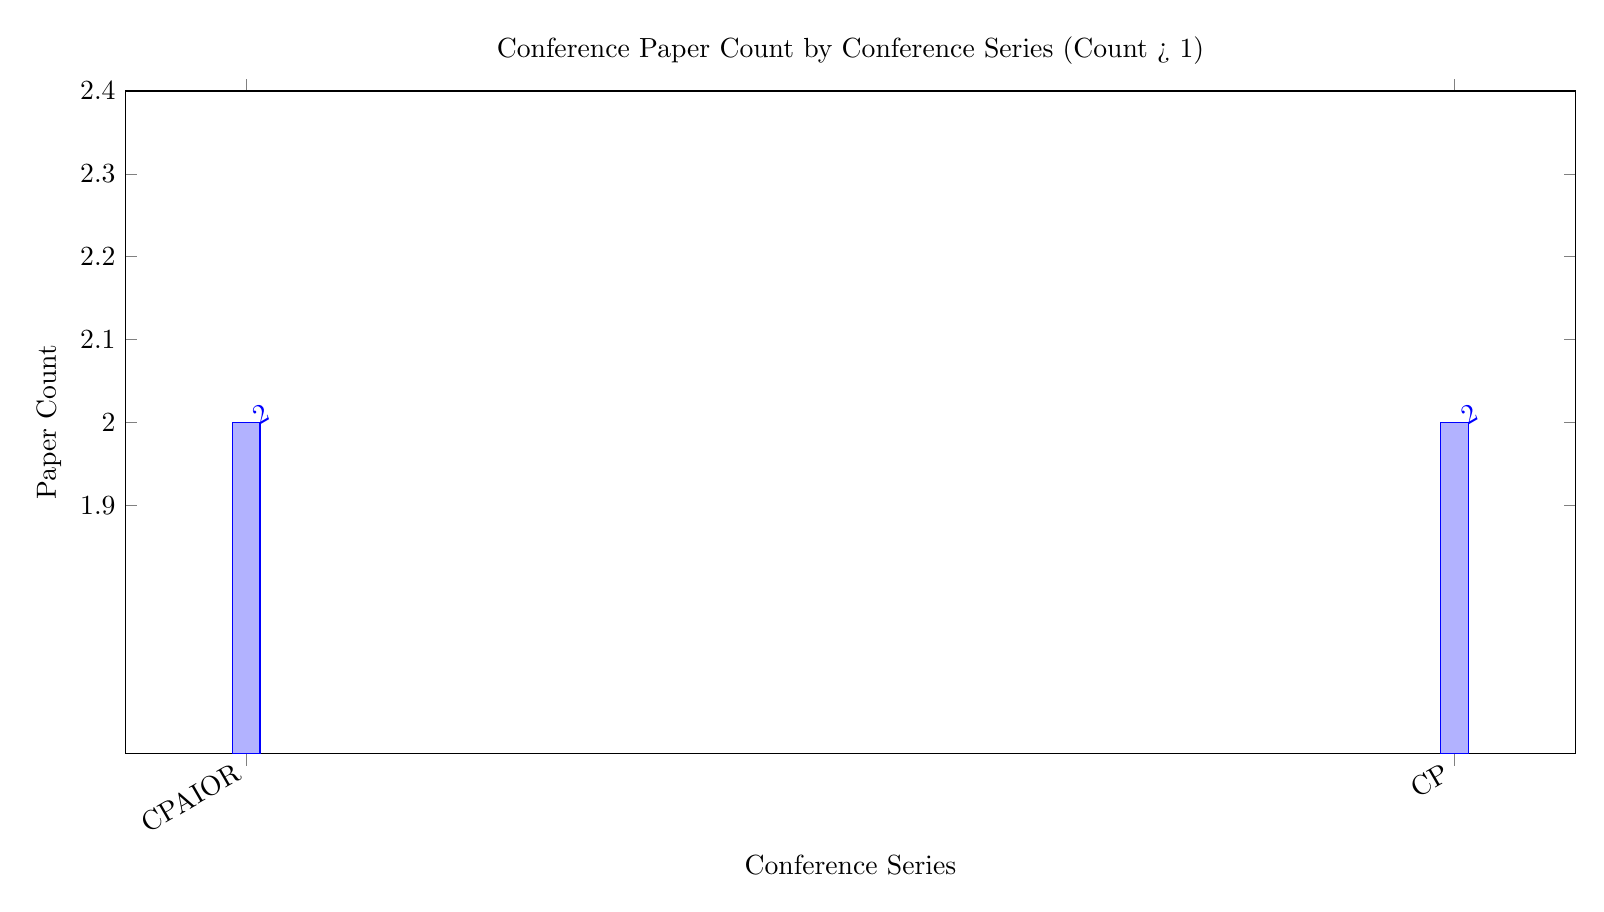
\begin{tikzpicture}
\begin{axis}[title=Conference Paper Count by Conference Series (Count > 1),xlabel=Conference Series,ylabel=Paper Count,
width=20cm,height=10cm,ybar,
symbolic x coords={CPAIOR,CP},
    xtick=data,nodes near coords, nodes near coords align={rotate=30),anchor=west},x tick label style={rotate=30),anchor=east}]
\addplot+[] coordinates {
(CPAIOR,2.000000)
(CP,2.000000)
};
\end{axis}
\end{tikzpicture}

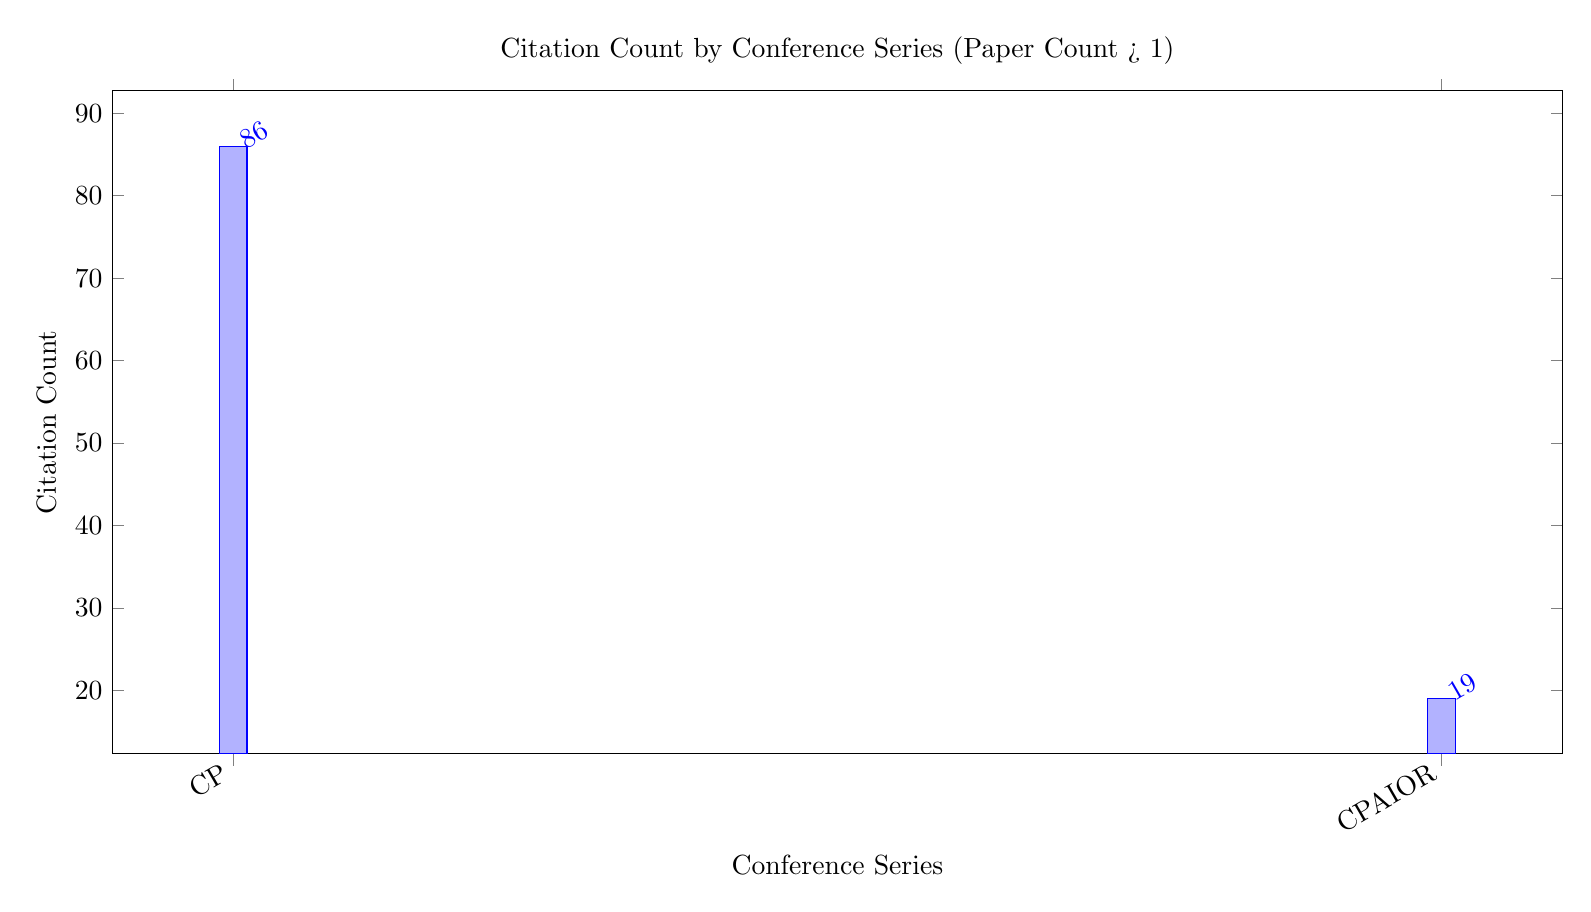
\begin{tikzpicture}
\begin{axis}[title=Citation Count by Conference Series (Paper Count > 1),xlabel=Conference Series,ylabel=Citation Count,
width=20cm,height=10cm,ybar,
symbolic x coords={CP,CPAIOR},
    xtick=data,nodes near coords, nodes near coords align={rotate=30),anchor=west},x tick label style={rotate=30),anchor=east}]
\addplot+[] coordinates {
(CP,86.000000)
(CPAIOR,19.000000)
};
\end{axis}
\end{tikzpicture}

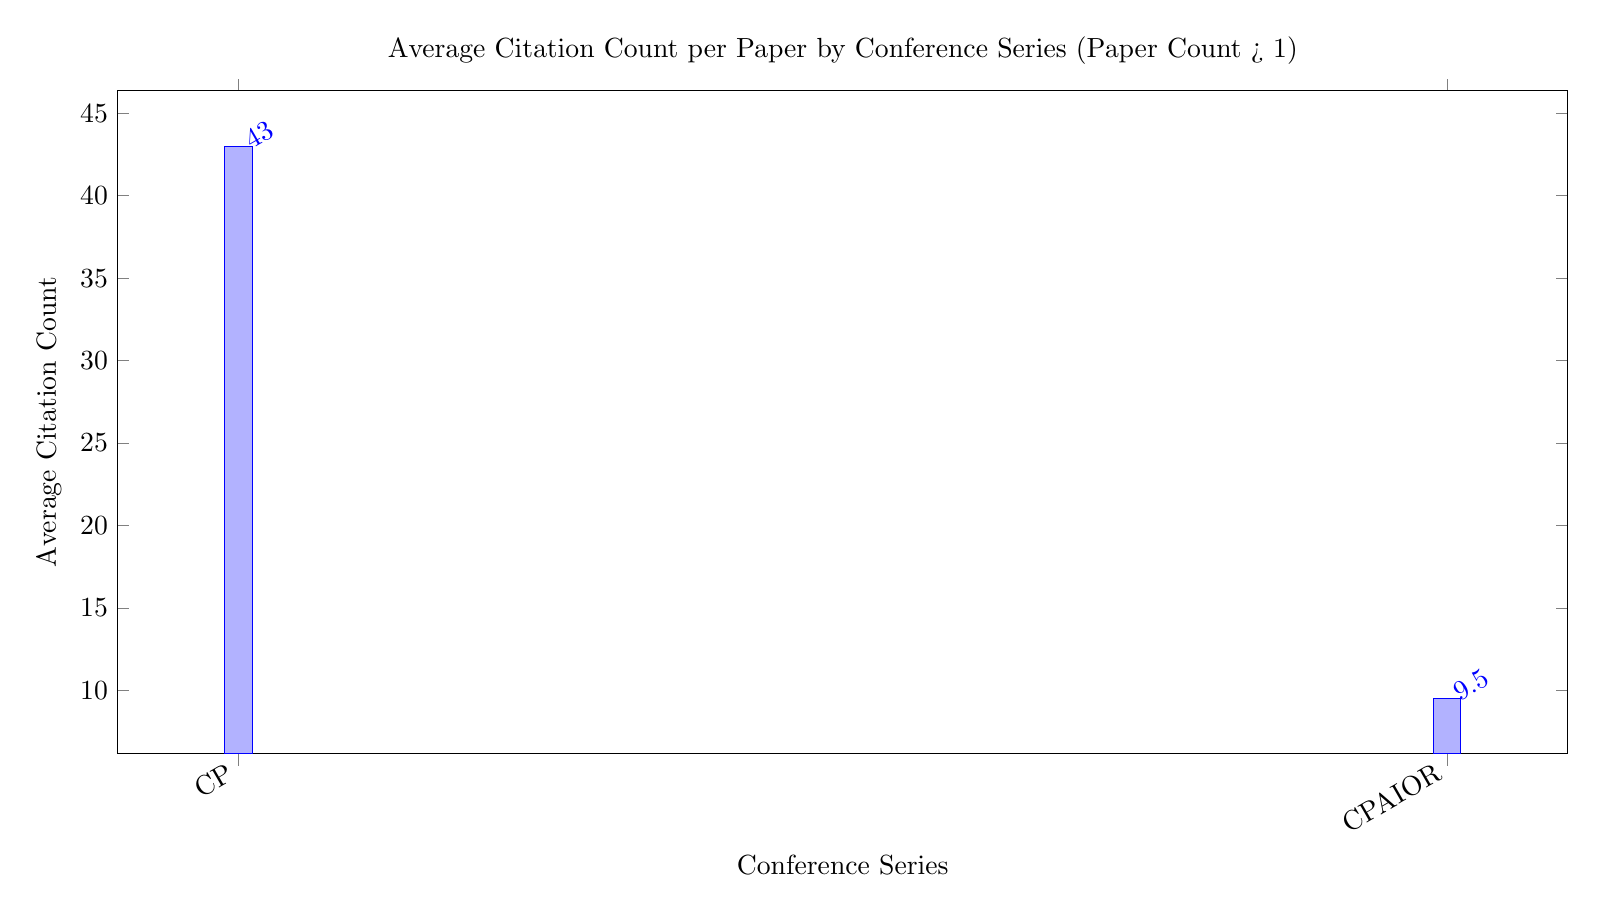
\begin{tikzpicture}
\begin{axis}[title=Average Citation Count per Paper by Conference Series (Paper Count > 1),xlabel=Conference Series,ylabel=Average Citation Count,
width=20cm,height=10cm,ybar,
symbolic x coords={CP,CPAIOR},
    xtick=data,nodes near coords, nodes near coords align={rotate=30),anchor=west},x tick label style={rotate=30),anchor=east}]
\addplot+[] coordinates {
(CP,43.000000)
(CPAIOR,9.500000)
};
\end{axis}
\end{tikzpicture}

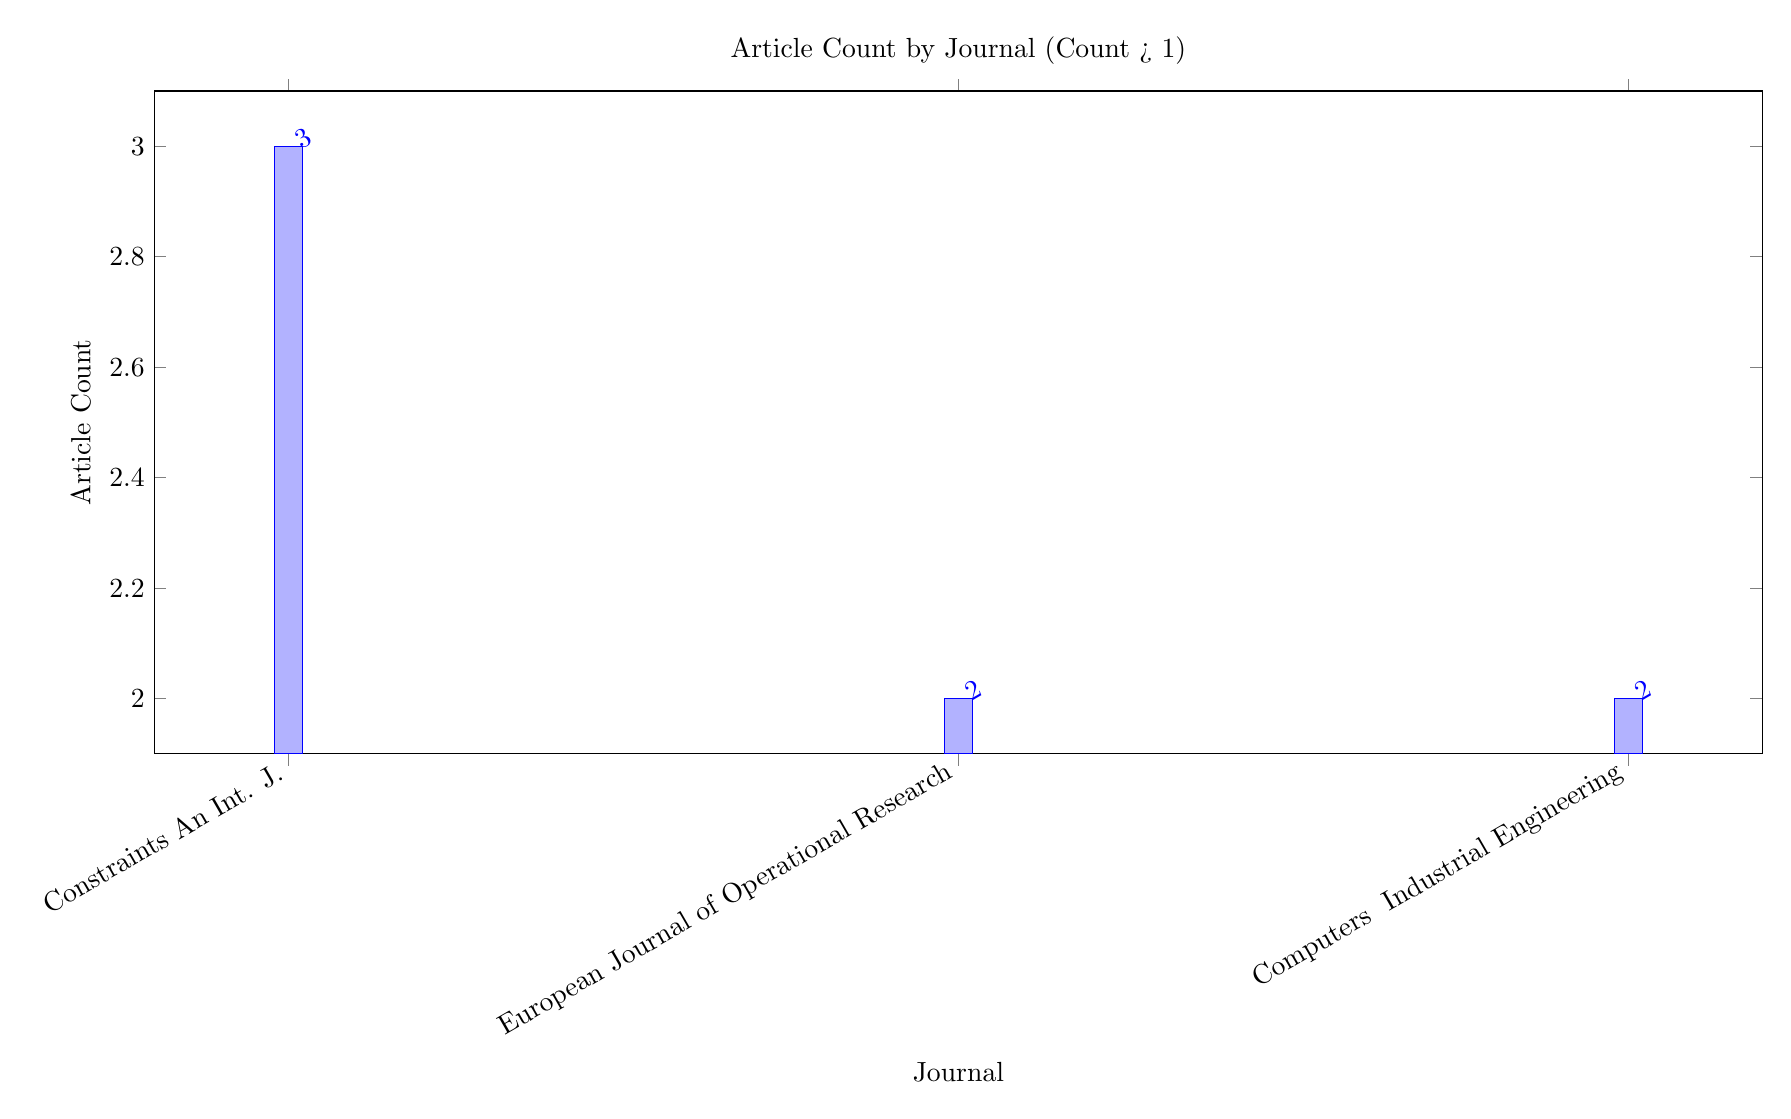
\begin{tikzpicture}
\begin{axis}[title=Article Count by Journal (Count > 1),xlabel=Journal,ylabel=Article Count,
width=22cm,height=10cm,ybar,
symbolic x coords={Constraints An Int. J.,European Journal of Operational Research,Computers \  Industrial Engineering},
    xtick=data,nodes near coords, nodes near coords align={rotate=30),anchor=west},x tick label style={rotate=30),anchor=east}]
\addplot+[] coordinates {
(Constraints An Int. J.,3.000000)
(European Journal of Operational Research,2.000000)
(Computers \  Industrial Engineering,2.000000)
};
\end{axis}
\end{tikzpicture}

\begin{tikzpicture}
\begin{axis}[title=Citation Count by Journal (Article Count > 1),xlabel=Journal,ylabel=Citation Count,
width=22cm,height=10cm,ybar,
symbolic x coords={European Journal of Operational Research,Constraints An Int. J.,Computers \  Industrial Engineering},
    xtick=data,nodes near coords, nodes near coords align={rotate=30),anchor=west},x tick label style={rotate=30),anchor=east}]
\addplot+[] coordinates {
(European Journal of Operational Research,454.000000)
(Constraints An Int. J.,47.000000)
(Computers \  Industrial Engineering,32.000000)
};
\end{axis}
\end{tikzpicture}

\begin{tikzpicture}
\begin{axis}[title=Average Citation Count per Article by Journal (Article Count > 1),xlabel=Journal,ylabel=Average Citation Count,
width=22cm,height=10cm,ybar,
symbolic x coords={European Journal of Operational Research,Computers \  Industrial Engineering,Constraints An Int. J.},
    xtick=data,nodes near coords, nodes near coords align={rotate=30),anchor=west},x tick label style={rotate=30),anchor=east}]
\addplot+[] coordinates {
(European Journal of Operational Research,227.000000)
(Computers \  Industrial Engineering,16.000000)
(Constraints An Int. J.,15.666667)
};
\end{axis}
\end{tikzpicture}

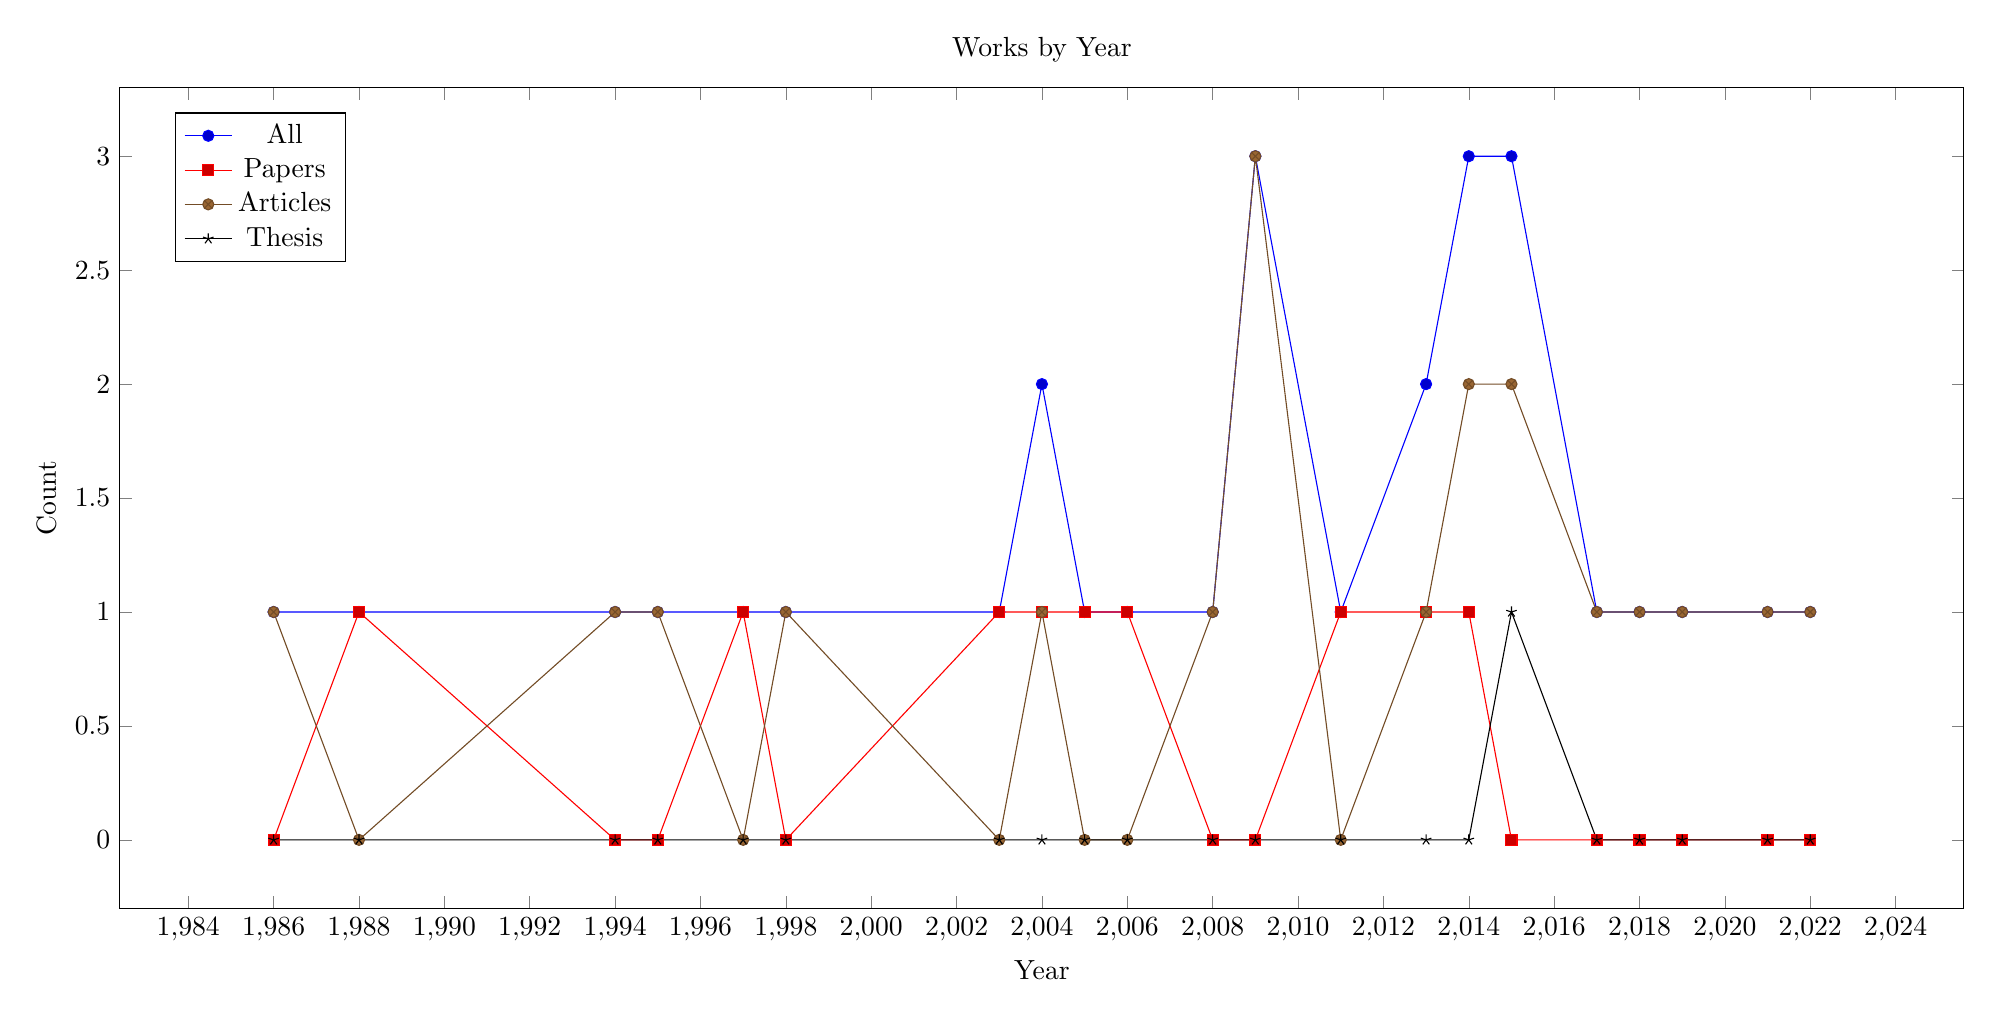
\begin{tikzpicture}
\begin{axis}[title=Works by Year,xlabel=Year,ylabel=Count,legend pos=north west,,width=25cm,height=12cm]
\addplot+[] coordinates {
    (1986.00,1.00000)
    (1988.00,1.00000)
    (1994.00,1.00000)
    (1995.00,1.00000)
    (1997.00,1.00000)
    (1998.00,1.00000)
    (2003.00,1.00000)
    (2004.00,2.00000)
    (2005.00,1.00000)
    (2006.00,1.00000)
    (2008.00,1.00000)
    (2009.00,3.00000)
    (2011.00,1.00000)
    (2013.00,2.00000)
    (2014.00,3.00000)
    (2015.00,3.00000)
    (2017.00,1.00000)
    (2018.00,1.00000)
    (2019.00,1.00000)
    (2021.00,1.00000)
    (2022.00,1.00000)
};
\addlegendentry{All}
\addplot+[] coordinates {
    (1986.00,0.00000)
    (1988.00,1.00000)
    (1994.00,0.00000)
    (1995.00,0.00000)
    (1997.00,1.00000)
    (1998.00,0.00000)
    (2003.00,1.00000)
    (2004.00,1.00000)
    (2005.00,1.00000)
    (2006.00,1.00000)
    (2008.00,0.00000)
    (2009.00,0.00000)
    (2011.00,1.00000)
    (2013.00,1.00000)
    (2014.00,1.00000)
    (2015.00,0.00000)
    (2017.00,0.00000)
    (2018.00,0.00000)
    (2019.00,0.00000)
    (2021.00,0.00000)
    (2022.00,0.00000)
};
\addlegendentry{Papers}
\addplot+[] coordinates {
    (1986.00,1.00000)
    (1988.00,0.00000)
    (1994.00,1.00000)
    (1995.00,1.00000)
    (1997.00,0.00000)
    (1998.00,1.00000)
    (2003.00,0.00000)
    (2004.00,1.00000)
    (2005.00,0.00000)
    (2006.00,0.00000)
    (2008.00,1.00000)
    (2009.00,3.00000)
    (2011.00,0.00000)
    (2013.00,1.00000)
    (2014.00,2.00000)
    (2015.00,2.00000)
    (2017.00,1.00000)
    (2018.00,1.00000)
    (2019.00,1.00000)
    (2021.00,1.00000)
    (2022.00,1.00000)
};
\addlegendentry{Articles}
\addplot+[] coordinates {
    (1986.00,0.00000)
    (1988.00,0.00000)
    (1994.00,0.00000)
    (1995.00,0.00000)
    (1997.00,0.00000)
    (1998.00,0.00000)
    (2003.00,0.00000)
    (2004.00,0.00000)
    (2005.00,0.00000)
    (2006.00,0.00000)
    (2008.00,0.00000)
    (2009.00,0.00000)
    (2011.00,0.00000)
    (2013.00,0.00000)
    (2014.00,0.00000)
    (2015.00,1.00000)
    (2017.00,0.00000)
    (2018.00,0.00000)
    (2019.00,0.00000)
    (2021.00,0.00000)
    (2022.00,0.00000)
};
\addlegendentry{Thesis}
\end{axis}
\end{tikzpicture}

\begin{tikzpicture}
\begin{axis}[title=Citations by Year,xlabel=Year,ylabel=Citations,legend pos=north west,,width=25cm,height=12cm]
\addplot+[] coordinates {
    (1986.00,74.0000)
    (1988.00,0.00000)
    (1994.00,24.0000)
    (1995.00,28.0000)
    (1997.00,53.0000)
    (1998.00,0.00000)
    (2003.00,46.0000)
    (2004.00,86.0000)
    (2005.00,0.00000)
    (2006.00,33.0000)
    (2008.00,146.000)
    (2009.00,321.000)
    (2011.00,0.00000)
    (2013.00,31.0000)
    (2014.00,20.0000)
    (2015.00,15.0000)
    (2017.00,3.00000)
    (2018.00,0.00000)
    (2019.00,8.00000)
    (2021.00,0.00000)
    (2022.00,2.00000)
};
\addlegendentry{All}
\addplot+[] coordinates {
    (1986.00,0.00000)
    (1988.00,0.00000)
    (1994.00,0.00000)
    (1995.00,0.00000)
    (1997.00,53.0000)
    (1998.00,0.00000)
    (2003.00,46.0000)
    (2004.00,17.0000)
    (2005.00,0.00000)
    (2006.00,33.0000)
    (2008.00,0.00000)
    (2009.00,0.00000)
    (2011.00,0.00000)
    (2013.00,0.00000)
    (2014.00,2.00000)
    (2015.00,0.00000)
    (2017.00,0.00000)
    (2018.00,0.00000)
    (2019.00,0.00000)
    (2021.00,0.00000)
    (2022.00,0.00000)
};
\addlegendentry{Papers}
\addplot+[] coordinates {
    (1986.00,74.0000)
    (1988.00,0.00000)
    (1994.00,24.0000)
    (1995.00,28.0000)
    (1997.00,0.00000)
    (1998.00,0.00000)
    (2003.00,0.00000)
    (2004.00,69.0000)
    (2005.00,0.00000)
    (2006.00,0.00000)
    (2008.00,146.000)
    (2009.00,321.000)
    (2011.00,0.00000)
    (2013.00,31.0000)
    (2014.00,18.0000)
    (2015.00,15.0000)
    (2017.00,3.00000)
    (2018.00,0.00000)
    (2019.00,8.00000)
    (2021.00,0.00000)
    (2022.00,2.00000)
};
\addlegendentry{Articles}
\end{axis}
\end{tikzpicture}

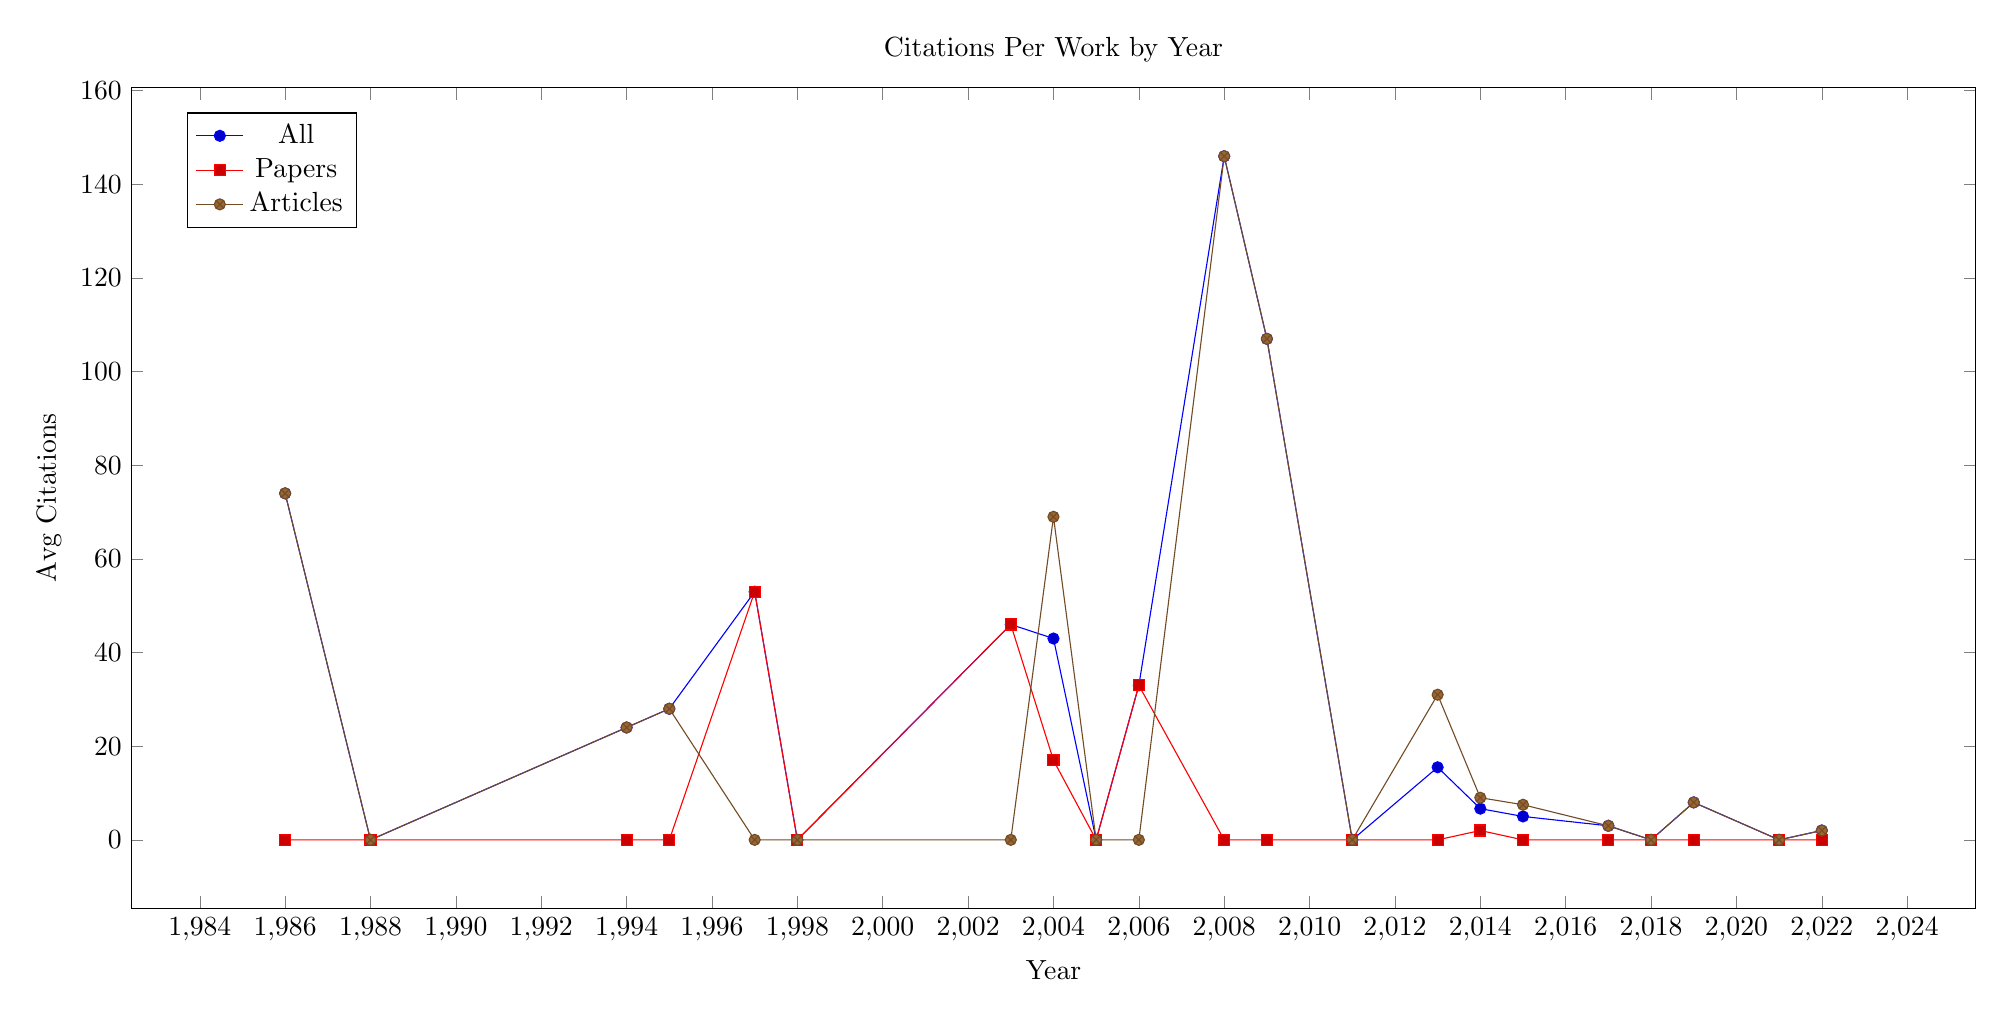
\begin{tikzpicture}
\begin{axis}[title=Citations Per Work by Year,xlabel=Year,ylabel=Avg Citations,legend pos=north west,,width=25cm,height=12cm]
\addplot+[] coordinates {
    (1986.00,74.0000)
    (1988.00,0.00000)
    (1994.00,24.0000)
    (1995.00,28.0000)
    (1997.00,53.0000)
    (1998.00,0.00000)
    (2003.00,46.0000)
    (2004.00,43.0000)
    (2005.00,0.00000)
    (2006.00,33.0000)
    (2008.00,146.000)
    (2009.00,107.000)
    (2011.00,0.00000)
    (2013.00,15.5000)
    (2014.00,6.66667)
    (2015.00,5.00000)
    (2017.00,3.00000)
    (2018.00,0.00000)
    (2019.00,8.00000)
    (2021.00,0.00000)
    (2022.00,2.00000)
};
\addlegendentry{All}
\addplot+[] coordinates {
    (1986.00,0.00000)
    (1988.00,0.00000)
    (1994.00,0.00000)
    (1995.00,0.00000)
    (1997.00,53.0000)
    (1998.00,0.00000)
    (2003.00,46.0000)
    (2004.00,17.0000)
    (2005.00,0.00000)
    (2006.00,33.0000)
    (2008.00,0.00000)
    (2009.00,0.00000)
    (2011.00,0.00000)
    (2013.00,0.00000)
    (2014.00,2.00000)
    (2015.00,0.00000)
    (2017.00,0.00000)
    (2018.00,0.00000)
    (2019.00,0.00000)
    (2021.00,0.00000)
    (2022.00,0.00000)
};
\addlegendentry{Papers}
\addplot+[] coordinates {
    (1986.00,74.0000)
    (1988.00,0.00000)
    (1994.00,24.0000)
    (1995.00,28.0000)
    (1997.00,0.00000)
    (1998.00,0.00000)
    (2003.00,0.00000)
    (2004.00,69.0000)
    (2005.00,0.00000)
    (2006.00,0.00000)
    (2008.00,146.000)
    (2009.00,107.000)
    (2011.00,0.00000)
    (2013.00,31.0000)
    (2014.00,9.00000)
    (2015.00,7.50000)
    (2017.00,3.00000)
    (2018.00,0.00000)
    (2019.00,8.00000)
    (2021.00,0.00000)
    (2022.00,2.00000)
};
\addlegendentry{Articles}
\end{axis}
\end{tikzpicture}

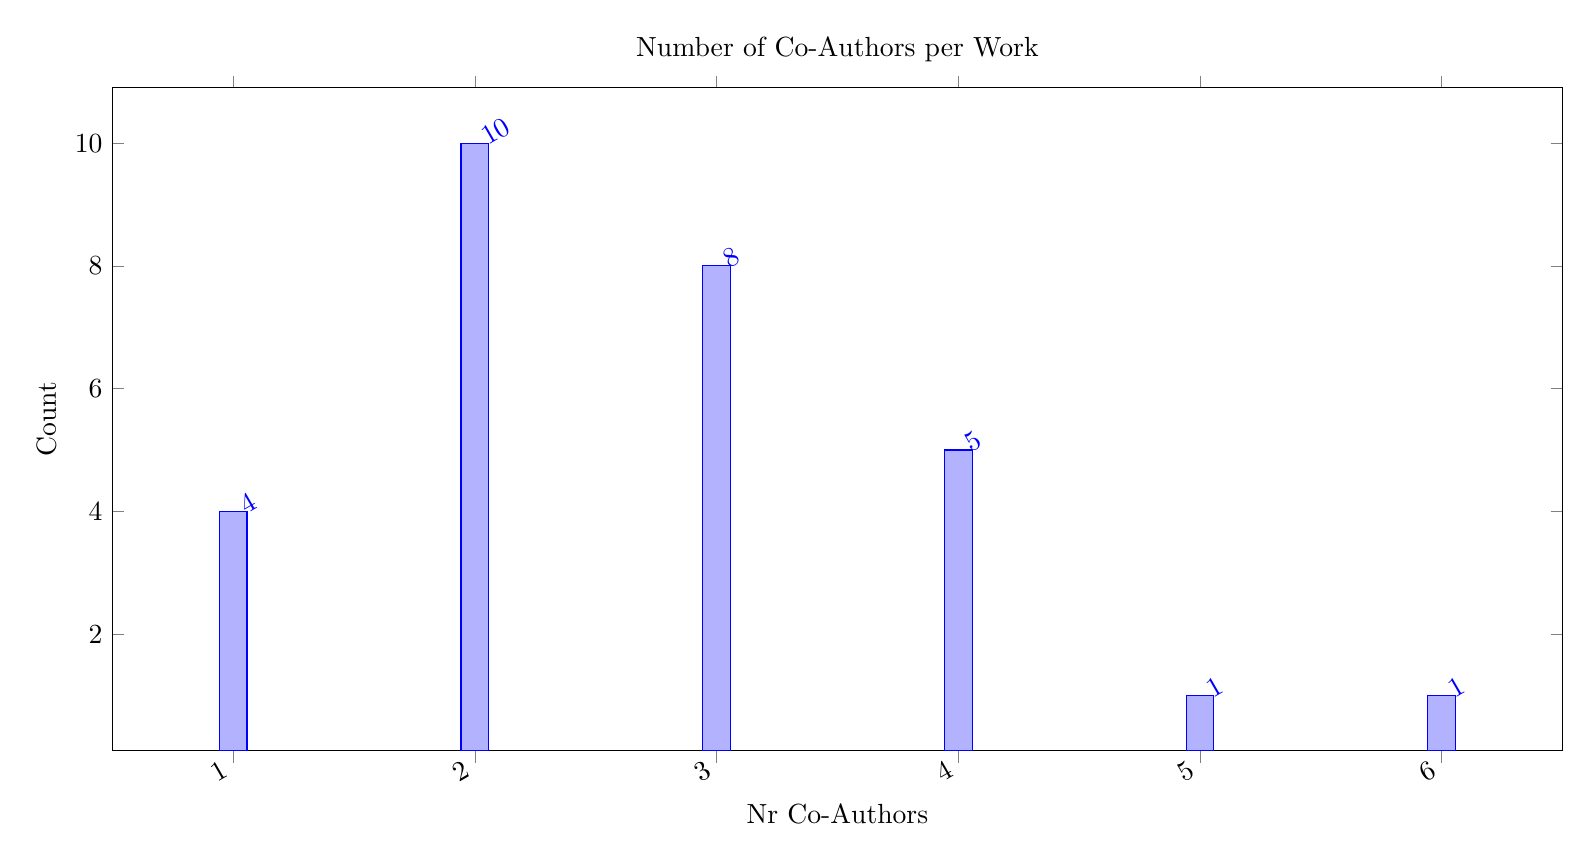
\begin{tikzpicture}
\begin{axis}[title=Number of Co-Authors per Work,xlabel=Nr Co-Authors,ylabel=Count,width=20cm,height=10cm,ybar,symbolic x coords={1,2,3,4,5,6},
    xtick=data,
    nodes near coords, 
    nodes near coords align={rotate=30,anchor=west},
    x tick label style={rotate=30,anchor=east},
]
\addplot+[] coordinates {
(1,4.000000)
(2,10.000000)
(3,8.000000)
(4,5.000000)
(5,1.000000)
(6,1.000000)
};
\end{axis}
\end{tikzpicture}

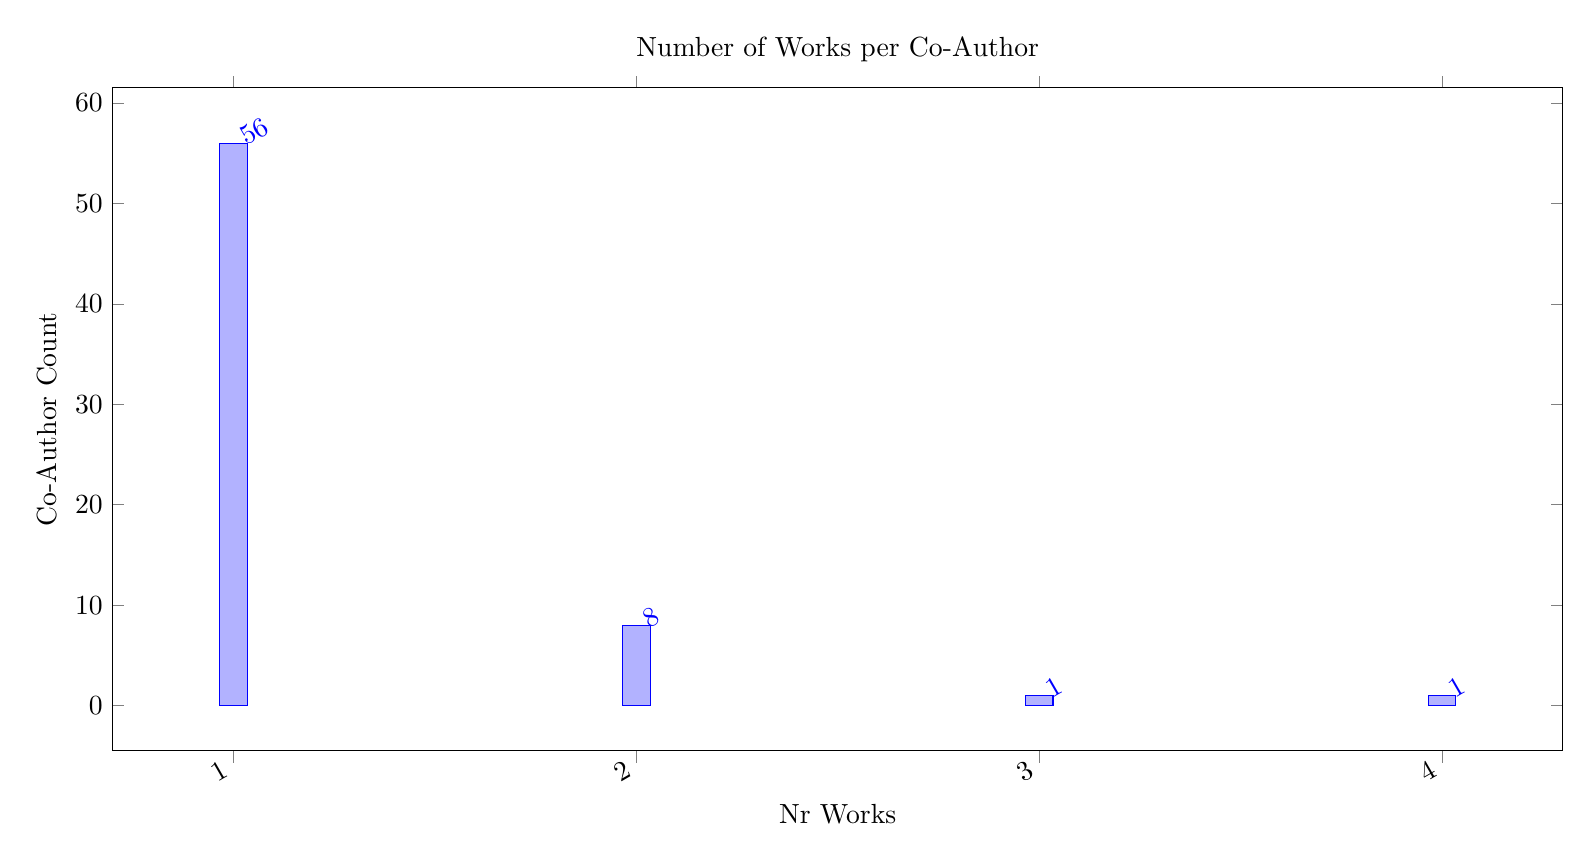
\begin{tikzpicture}
\begin{axis}[title=Number of Works per Co-Author,xlabel=Nr Works,ylabel=Co-Author Count,width=20cm,height=10cm,ybar,symbolic x coords={1,2,3,4},
    xtick=data,
    nodes near coords, 
    nodes near coords align={rotate=30,anchor=west},
    x tick label style={rotate=30,anchor=east},
]
\addplot+[] coordinates {
(1,56.000000)
(2,8.000000)
(3,1.000000)
(4,1.000000)
};
\end{axis}
\end{tikzpicture}

\begin{tikzpicture}
\begin{axis}[title=Nr Citation Distribution Plot ,xlabel=Nr Citations,ylabel=Nr Works,,width=25cm,height=15cm]
\addplot+[] coordinates {
    (2.00000,2.00000)
    (3.00000,2.00000)
    (8.00000,1.00000)
    (13.0000,1.00000)
    (15.0000,2.00000)
    (17.0000,1.00000)
    (24.0000,1.00000)
    (28.0000,1.00000)
    (31.0000,1.00000)
    (33.0000,1.00000)
    (46.0000,1.00000)
    (53.0000,1.00000)
    (69.0000,1.00000)
    (74.0000,1.00000)
    (146.000,1.00000)
};
\end{axis}
\end{tikzpicture}

\begin{table}[htbp]
\caption{Similarity Measure (*1000) based on References and Citations (high = similar)}
\centering
{\scriptsize
{\setlength{\tabcolsep}{2pt}
\begin{tabular}{lr|*{22}{@{ }r@{ }}|r}\toprule
From/To& \rotatebox{90}{Total}& \rotatebox{90}{SolnonCNA08}& \rotatebox{90}{SialaHH155}& \rotatebox{90}{GolleRB14}& \rotatebox{90}{Kis04}& \rotatebox{90}{ZhangGWH17}& \rotatebox{90}{PerronS04}& \rotatebox{90}{HoevePRS09}& \rotatebox{90}{SialaHH14}& \rotatebox{90}{GottliebPS03}& \rotatebox{90}{HoevePRS06}& \rotatebox{90}{MoyaCB19}& \rotatebox{90}{YuLZCLW22}& \rotatebox{90}{ArtiguesHM0W14}& \rotatebox{90}{ReginP97}& \rotatebox{90}{ParrelloK86}& \rotatebox{90}{WarwickT95}& \rotatebox{90}{BoysenFS09}& \rotatebox{90}{HindiP94}& \rotatebox{90}{OzturkTHO13}& \rotatebox{90}{Siala15}& \rotatebox{90}{Mayer-EichbergerW13}& \rotatebox{90}{Schaus09}& \rotatebox{90}{Other}\\ 
Total & & 4,744& 4,560& 4,108& 3,586& 3,468& 3,299& 3,261& 3,224& 3,156& 2,824& 2,410& 2,317& 2,103& 2,091& 1,841& 1,563& 1,552& 1,520& 407& 0& 0& 0& \\ 
\midrule
SolnonCNA08 & 4,744&0&\cellcolor{percentColor20!40}287&\cellcolor{percentColor50!40}586&\cellcolor{percentColor50!40}659&\cellcolor{percentColor30!40}434&\cellcolor{percentColor20!40}227&\cellcolor{percentColor10!40}130&\cellcolor{percentColor10!40}194&\cellcolor{percentColor20!40}293&\cellcolor{percentColor0!40}67&\cellcolor{percentColor30!40}385&\cellcolor{percentColor30!40}373&\cellcolor{percentColor0!40}66&\cellcolor{percentColor10!40}121&\cellcolor{percentColor20!40}309&\cellcolor{percentColor10!40}149&\cellcolor{percentColor20!40}328&\cellcolor{percentColor0!40}106&\cellcolor{percentColor0!40}30&0&0&0& 0\\ 
SialaHH155 & 4,560&\cellcolor{percentColor20!40}287&0&\cellcolor{percentColor50!40}640&\cellcolor{percentColor10!40}143&\cellcolor{percentColor40!40}508&\cellcolor{percentColor20!40}273&\cellcolor{percentColor10!40}183&\cellcolor{percentColor40!40}500&\cellcolor{percentColor20!40}232&\cellcolor{percentColor10!40}159&\cellcolor{percentColor20!40}248&\cellcolor{percentColor10!40}213&\cellcolor{percentColor50!40}579&\cellcolor{percentColor0!40}59&\cellcolor{percentColor10!40}157&\cellcolor{percentColor10!40}140&\cellcolor{percentColor0!40}93&\cellcolor{percentColor0!40}103&\cellcolor{percentColor0!40}43&0&0&0& 0\\ 
GolleRB14 & 4,108&\cellcolor{percentColor50!40}586&\cellcolor{percentColor50!40}640&0&\cellcolor{percentColor20!40}254&\cellcolor{percentColor50!40}648&\cellcolor{percentColor10!40}208&0&\cellcolor{percentColor10!40}138&\cellcolor{percentColor10!40}198&0&\cellcolor{percentColor30!40}392&\cellcolor{percentColor20!40}308&\cellcolor{percentColor10!40}182&\cellcolor{percentColor0!40}29&\cellcolor{percentColor10!40}135&\cellcolor{percentColor10!40}140&\cellcolor{percentColor10!40}113&\cellcolor{percentColor0!40}103&\cellcolor{percentColor0!40}34&0&0&0& 0\\ 
Kis04 & 3,586&\cellcolor{percentColor50!40}659&\cellcolor{percentColor10!40}143&\cellcolor{percentColor20!40}254&0&\cellcolor{percentColor10!40}170&\cellcolor{percentColor40!40}519&\cellcolor{percentColor0!40}24&\cellcolor{percentColor0!40}28&\cellcolor{percentColor30!40}348&\cellcolor{percentColor0!40}59&\cellcolor{percentColor0!40}95&\cellcolor{percentColor0!40}100&\cellcolor{percentColor0!40}28&\cellcolor{percentColor10!40}131&\cellcolor{percentColor30!40}406&\cellcolor{percentColor20!40}309&\cellcolor{percentColor10!40}119&\cellcolor{percentColor10!40}151&\cellcolor{percentColor0!40}43&0&0&0& 0\\ 
ZhangGWH17 & 3,468&\cellcolor{percentColor30!40}434&\cellcolor{percentColor40!40}508&\cellcolor{percentColor50!40}648&\cellcolor{percentColor10!40}170&0&\cellcolor{percentColor10!40}146&\cellcolor{percentColor0!40}50&\cellcolor{percentColor10!40}174&\cellcolor{percentColor0!40}54&\cellcolor{percentColor0!40}51&\cellcolor{percentColor30!40}395&\cellcolor{percentColor30!40}406&\cellcolor{percentColor10!40}125&0&\cellcolor{percentColor0!40}52&\cellcolor{percentColor0!40}65&\cellcolor{percentColor10!40}137&0&\cellcolor{percentColor0!40}53&0&0&0& 0\\ 
PerronS04 & 3,299&\cellcolor{percentColor20!40}227&\cellcolor{percentColor20!40}273&\cellcolor{percentColor10!40}208&\cellcolor{percentColor40!40}519&\cellcolor{percentColor10!40}146&0&\cellcolor{percentColor20!40}251&\cellcolor{percentColor10!40}187&\cellcolor{percentColor30!40}333&\cellcolor{percentColor10!40}205&\cellcolor{percentColor0!40}38&\cellcolor{percentColor0!40}87&\cellcolor{percentColor20!40}291&\cellcolor{percentColor10!40}171&\cellcolor{percentColor0!40}88&\cellcolor{percentColor0!40}89&\cellcolor{percentColor0!40}40&\cellcolor{percentColor10!40}146&0&0&0&0& 0\\ 
HoevePRS09 & 3,261&\cellcolor{percentColor10!40}130&\cellcolor{percentColor10!40}183&0&\cellcolor{percentColor0!40}24&\cellcolor{percentColor0!40}50&\cellcolor{percentColor20!40}251&0&\cellcolor{percentColor60!40}705&\cellcolor{percentColor10!40}188&\cellcolor{percentColor90!40}1,104&0&0&\cellcolor{percentColor0!40}83&\cellcolor{percentColor30!40}424&0&0&\cellcolor{percentColor0!40}11&\cellcolor{percentColor0!40}108&0&0&0&0& 0\\ 
SialaHH14 & 3,224&\cellcolor{percentColor10!40}194&\cellcolor{percentColor40!40}500&\cellcolor{percentColor10!40}138&\cellcolor{percentColor0!40}28&\cellcolor{percentColor10!40}174&\cellcolor{percentColor10!40}187&\cellcolor{percentColor60!40}705&0&\cellcolor{percentColor10!40}146&\cellcolor{percentColor20!40}286&\cellcolor{percentColor0!40}69&\cellcolor{percentColor10!40}157&\cellcolor{percentColor30!40}333&\cellcolor{percentColor10!40}189&0&0&\cellcolor{percentColor0!40}44&\cellcolor{percentColor0!40}74&0&0&0&0& 0\\ 
GottliebPS03 & 3,156&\cellcolor{percentColor20!40}293&\cellcolor{percentColor20!40}232&\cellcolor{percentColor10!40}198&\cellcolor{percentColor30!40}348&\cellcolor{percentColor0!40}54&\cellcolor{percentColor30!40}333&\cellcolor{percentColor10!40}188&\cellcolor{percentColor10!40}146&0&\cellcolor{percentColor10!40}217&\cellcolor{percentColor0!40}78&\cellcolor{percentColor0!40}95&\cellcolor{percentColor10!40}137&\cellcolor{percentColor10!40}182&\cellcolor{percentColor20!40}233&\cellcolor{percentColor10!40}216&\cellcolor{percentColor0!40}63&\cellcolor{percentColor10!40}143&0&0&0&0& 0\\ 
HoevePRS06 & 2,824&\cellcolor{percentColor0!40}67&\cellcolor{percentColor10!40}159&0&\cellcolor{percentColor0!40}59&\cellcolor{percentColor0!40}51&\cellcolor{percentColor10!40}205&\cellcolor{percentColor90!40}1,104&\cellcolor{percentColor20!40}286&\cellcolor{percentColor10!40}217&0&0&0&\cellcolor{percentColor0!40}87&\cellcolor{percentColor40!40}456&\cellcolor{percentColor0!40}19&\cellcolor{percentColor0!40}33&\cellcolor{percentColor0!40}11&\cellcolor{percentColor0!40}70&0&0&0&0& 0\\ 
MoyaCB19 & 2,410&\cellcolor{percentColor30!40}385&\cellcolor{percentColor20!40}248&\cellcolor{percentColor30!40}392&\cellcolor{percentColor0!40}95&\cellcolor{percentColor30!40}395&\cellcolor{percentColor0!40}38&0&\cellcolor{percentColor0!40}69&\cellcolor{percentColor0!40}78&0&0&\cellcolor{percentColor30!40}370&\cellcolor{percentColor0!40}33&0&\cellcolor{percentColor0!40}73&\cellcolor{percentColor0!40}56&\cellcolor{percentColor0!40}92&\cellcolor{percentColor0!40}63&\cellcolor{percentColor0!40}23&0&0&0& 0\\ 
YuLZCLW22 & 2,317&\cellcolor{percentColor30!40}373&\cellcolor{percentColor10!40}213&\cellcolor{percentColor20!40}308&\cellcolor{percentColor0!40}100&\cellcolor{percentColor30!40}406&\cellcolor{percentColor0!40}87&0&\cellcolor{percentColor10!40}157&\cellcolor{percentColor0!40}95&0&\cellcolor{percentColor30!40}370&0&\cellcolor{percentColor0!40}75&0&0&0&\cellcolor{percentColor0!40}108&0&\cellcolor{percentColor0!40}25&0&0&0& 0\\ 
ArtiguesHM0W14 & 2,103&\cellcolor{percentColor0!40}66&\cellcolor{percentColor50!40}579&\cellcolor{percentColor10!40}182&\cellcolor{percentColor0!40}28&\cellcolor{percentColor10!40}125&\cellcolor{percentColor20!40}291&\cellcolor{percentColor0!40}83&\cellcolor{percentColor30!40}333&\cellcolor{percentColor10!40}137&\cellcolor{percentColor0!40}87&\cellcolor{percentColor0!40}33&\cellcolor{percentColor0!40}75&0&\cellcolor{percentColor0!40}36&\cellcolor{percentColor0!40}26&0&\cellcolor{percentColor0!40}22&0&0&0&0&0& 0\\ 
ReginP97 & 2,091&\cellcolor{percentColor10!40}121&\cellcolor{percentColor0!40}59&\cellcolor{percentColor0!40}29&\cellcolor{percentColor10!40}131&0&\cellcolor{percentColor10!40}171&\cellcolor{percentColor30!40}424&\cellcolor{percentColor10!40}189&\cellcolor{percentColor10!40}182&\cellcolor{percentColor40!40}456&0&0&\cellcolor{percentColor0!40}36&0&\cellcolor{percentColor0!40}110&\cellcolor{percentColor0!40}99&\cellcolor{percentColor0!40}6&\cellcolor{percentColor0!40}78&0&0&0&0& 0\\ 
ParrelloK86 & 1,841&\cellcolor{percentColor20!40}309&\cellcolor{percentColor10!40}157&\cellcolor{percentColor10!40}135&\cellcolor{percentColor30!40}406&\cellcolor{percentColor0!40}52&\cellcolor{percentColor0!40}88&0&0&\cellcolor{percentColor20!40}233&\cellcolor{percentColor0!40}19&\cellcolor{percentColor0!40}73&0&\cellcolor{percentColor0!40}26&\cellcolor{percentColor0!40}110&0&0&\cellcolor{percentColor10!40}131&\cellcolor{percentColor0!40}102&0&0&0&0& 0\\ 
WarwickT95 & 1,563&\cellcolor{percentColor10!40}149&\cellcolor{percentColor10!40}140&\cellcolor{percentColor10!40}140&\cellcolor{percentColor20!40}309&\cellcolor{percentColor0!40}65&\cellcolor{percentColor0!40}89&0&0&\cellcolor{percentColor10!40}216&\cellcolor{percentColor0!40}33&\cellcolor{percentColor0!40}56&0&0&\cellcolor{percentColor0!40}99&0&0&\cellcolor{percentColor0!40}36&\cellcolor{percentColor20!40}231&0&0&0&0& 0\\ 
BoysenFS09 & 1,552&\cellcolor{percentColor20!40}328&\cellcolor{percentColor0!40}93&\cellcolor{percentColor10!40}113&\cellcolor{percentColor10!40}119&\cellcolor{percentColor10!40}137&\cellcolor{percentColor0!40}40&\cellcolor{percentColor0!40}11&\cellcolor{percentColor0!40}44&\cellcolor{percentColor0!40}63&\cellcolor{percentColor0!40}11&\cellcolor{percentColor0!40}92&\cellcolor{percentColor0!40}108&\cellcolor{percentColor0!40}22&\cellcolor{percentColor0!40}6&\cellcolor{percentColor10!40}131&\cellcolor{percentColor0!40}36&0&\cellcolor{percentColor0!40}42&\cellcolor{percentColor10!40}156&0&0&0& 0\\ 
HindiP94 & 1,520&\cellcolor{percentColor0!40}106&\cellcolor{percentColor0!40}103&\cellcolor{percentColor0!40}103&\cellcolor{percentColor10!40}151&0&\cellcolor{percentColor10!40}146&\cellcolor{percentColor0!40}108&\cellcolor{percentColor0!40}74&\cellcolor{percentColor10!40}143&\cellcolor{percentColor0!40}70&\cellcolor{percentColor0!40}63&0&0&\cellcolor{percentColor0!40}78&\cellcolor{percentColor0!40}102&\cellcolor{percentColor20!40}231&\cellcolor{percentColor0!40}42&0&0&0&0&0& 0\\ 
OzturkTHO13 & 407&\cellcolor{percentColor0!40}30&\cellcolor{percentColor0!40}43&\cellcolor{percentColor0!40}34&\cellcolor{percentColor0!40}43&\cellcolor{percentColor0!40}53&0&0&0&0&0&\cellcolor{percentColor0!40}23&\cellcolor{percentColor0!40}25&0&0&0&0&\cellcolor{percentColor10!40}156&0&0&0&0&0& 0\\ 
Siala15 & 0&0&0&0&0&0&0&0&0&0&0&0&0&0&0&0&0&0&0&0&0&0&0& 0\\ 
Mayer-EichbergerW13 & 0&0&0&0&0&0&0&0&0&0&0&0&0&0&0&0&0&0&0&0&0&0&0& 0\\ 
Schaus09 & 0&0&0&0&0&0&0&0&0&0&0&0&0&0&0&0&0&0&0&0&0&0&0& 0\\ 
Gent98 & 0&0&0&0&0&0&0&0&0&0&0&0&0&0&0&0&0&0&0&0&0&0&0& 0\\ 
ButaruH05 & 0&0&0&0&0&0&0&0&0&0&0&0&0&0&0&0&0&0&0&0&0&0&0& 0\\ 
YavuzE18 & 0&0&0&0&0&0&0&0&0&0&0&0&0&0&0&0&0&0&0&0&0&0&0& 0\\ 
WinterM21 & 0&0&0&0&0&0&0&0&0&0&0&0&0&0&0&0&0&0&0&0&0&0&0& 0\\ 
DincbasSH88 & 0&0&0&0&0&0&0&0&0&0&0&0&0&0&0&0&0&0&0&0&0&0&0& 0\\ 
ThiruvadyME11 & 0&0&0&0&0&0&0&0&0&0&0&0&0&0&0&0&0&0&0&0&0&0&0& 0\\ 
MazurN15 & 0&0&0&0&0&0&0&0&0&0&0&0&0&0&0&0&0&0&0&0&0&0&0& 0\\ 
\midrule
Other & & 0& 0& 0& 0& 0& 0& 0& 0& 0& 0& 0& 0& 0& 0& 0& 0& 0& 0& 0& 0& 0& 0\\ 
\bottomrule
\end{tabular}
}
}
\end{table}

\begin{table}[htbp]
\caption{Similarity Measure based on Extracted Concepts (low = similar)}
\centering
{\scriptsize
{\setlength{\tabcolsep}{2pt}
\begin{tabular}{lr|*{35}{@{ }r@{ }}|r}\toprule
From/To& \rotatebox{90}{Total}& \rotatebox{90}{Siala15}& \rotatebox{90}{OzturkTHO13}& \rotatebox{90}{BoysenFS09}& \rotatebox{90}{DincbasSH88}& \rotatebox{90}{SialaHH14}& \rotatebox{90}{YuLZCLW22}& \rotatebox{90}{MoyaCB19}& \rotatebox{90}{ParrelloK86}& \rotatebox{90}{SialaHH155}& \rotatebox{90}{HoevePRS09}& \rotatebox{90}{Mayer-EichbergerW13}& \rotatebox{90}{SolnonCNA08}& \rotatebox{90}{HoevePRS06}& \rotatebox{90}{ArtiguesHM0W14}& \rotatebox{90}{ReginP97}& \rotatebox{90}{ZhangGWH17}& \rotatebox{90}{GottliebPS03}& \rotatebox{90}{PerronS04}& \rotatebox{90}{Kis04}& \rotatebox{90}{ButaruH05}& \rotatebox{90}{GolleRB14}& \rotatebox{90}{Other}\\ 
Total & & 315& 248& 215& 204& 197& 190& 175& 170& 166& 165& 163& 161& 161& 158& 156& 154& 149& 144& 143& 142& 142& \\ 
\midrule
Siala15 & 315&0&\cellcolor{percentColor80!40}15&\cellcolor{percentColor90!40}16&\cellcolor{percentColor90!40}16&\cellcolor{percentColor80!40}14&\cellcolor{percentColor90!40}17&\cellcolor{percentColor90!40}16&\cellcolor{percentColor90!40}16&\cellcolor{percentColor80!40}15&\cellcolor{percentColor80!40}15&\cellcolor{percentColor90!40}16&\cellcolor{percentColor90!40}16&\cellcolor{percentColor90!40}16&\cellcolor{percentColor80!40}15&\cellcolor{percentColor90!40}16&\cellcolor{percentColor90!40}16&\cellcolor{percentColor90!40}16&\cellcolor{percentColor90!40}16&\cellcolor{percentColor90!40}16&\cellcolor{percentColor90!40}16&\cellcolor{percentColor90!40}16& 0\\ 
OzturkTHO13 & 248&\cellcolor{percentColor80!40}15&0&\cellcolor{percentColor60!40}11&\cellcolor{percentColor50!40}10&\cellcolor{percentColor80!40}15&\cellcolor{percentColor70!40}12&\cellcolor{percentColor70!40}13&\cellcolor{percentColor70!40}12&\cellcolor{percentColor70!40}13&\cellcolor{percentColor70!40}13&\cellcolor{percentColor70!40}13&\cellcolor{percentColor70!40}12&\cellcolor{percentColor70!40}13&\cellcolor{percentColor70!40}13&\cellcolor{percentColor70!40}12&\cellcolor{percentColor70!40}12&\cellcolor{percentColor70!40}12&\cellcolor{percentColor60!40}11&\cellcolor{percentColor70!40}12&\cellcolor{percentColor70!40}12&\cellcolor{percentColor70!40}12& 0\\ 
BoysenFS09 & 215&\cellcolor{percentColor90!40}16&\cellcolor{percentColor60!40}11&0&\cellcolor{percentColor60!40}11&\cellcolor{percentColor70!40}13&\cellcolor{percentColor50!40}10&\cellcolor{percentColor50!40}10&\cellcolor{percentColor50!40}10&\cellcolor{percentColor60!40}11&\cellcolor{percentColor60!40}11&\cellcolor{percentColor60!40}11&\cellcolor{percentColor50!40}10&\cellcolor{percentColor60!40}11&\cellcolor{percentColor60!40}11&\cellcolor{percentColor50!40}10&\cellcolor{percentColor50!40}10&\cellcolor{percentColor50!40}10&\cellcolor{percentColor50!40}10&\cellcolor{percentColor50!40}10&\cellcolor{percentColor50!40}10&\cellcolor{percentColor50!40}9& 0\\ 
DincbasSH88 & 204&\cellcolor{percentColor90!40}16&\cellcolor{percentColor50!40}10&\cellcolor{percentColor60!40}11&0&\cellcolor{percentColor70!40}12&\cellcolor{percentColor60!40}11&\cellcolor{percentColor60!40}11&\cellcolor{percentColor40!40}8&\cellcolor{percentColor50!40}10&\cellcolor{percentColor50!40}10&\cellcolor{percentColor60!40}11&\cellcolor{percentColor50!40}9&\cellcolor{percentColor50!40}10&\cellcolor{percentColor60!40}11&\cellcolor{percentColor50!40}9&\cellcolor{percentColor50!40}10&\cellcolor{percentColor50!40}10&\cellcolor{percentColor40!40}8&\cellcolor{percentColor50!40}9&\cellcolor{percentColor50!40}9&\cellcolor{percentColor50!40}9& 0\\ 
SialaHH14 & 197&\cellcolor{percentColor80!40}14&\cellcolor{percentColor80!40}15&\cellcolor{percentColor70!40}13&\cellcolor{percentColor70!40}12&0&\cellcolor{percentColor60!40}11&\cellcolor{percentColor50!40}10&\cellcolor{percentColor60!40}11&\cellcolor{percentColor40!40}7&\cellcolor{percentColor40!40}7&\cellcolor{percentColor40!40}8&\cellcolor{percentColor50!40}10&\cellcolor{percentColor40!40}8&\cellcolor{percentColor40!40}8&\cellcolor{percentColor50!40}9&\cellcolor{percentColor50!40}9&\cellcolor{percentColor50!40}9&\cellcolor{percentColor50!40}9&\cellcolor{percentColor50!40}9&\cellcolor{percentColor50!40}9&\cellcolor{percentColor50!40}9& 0\\ 
YuLZCLW22 & 190&\cellcolor{percentColor90!40}17&\cellcolor{percentColor70!40}12&\cellcolor{percentColor50!40}10&\cellcolor{percentColor60!40}11&\cellcolor{percentColor60!40}11&0&\cellcolor{percentColor50!40}9&\cellcolor{percentColor50!40}9&\cellcolor{percentColor50!40}9&\cellcolor{percentColor50!40}10&\cellcolor{percentColor50!40}9&\cellcolor{percentColor40!40}8&\cellcolor{percentColor50!40}10&\cellcolor{percentColor50!40}9&\cellcolor{percentColor50!40}9&\cellcolor{percentColor40!40}7&\cellcolor{percentColor40!40}8&\cellcolor{percentColor40!40}8&\cellcolor{percentColor40!40}8&\cellcolor{percentColor40!40}8&\cellcolor{percentColor40!40}8& 0\\ 
MoyaCB19 & 175&\cellcolor{percentColor90!40}16&\cellcolor{percentColor70!40}13&\cellcolor{percentColor50!40}10&\cellcolor{percentColor60!40}11&\cellcolor{percentColor50!40}10&\cellcolor{percentColor50!40}9&0&\cellcolor{percentColor50!40}9&\cellcolor{percentColor40!40}8&\cellcolor{percentColor50!40}9&\cellcolor{percentColor40!40}8&\cellcolor{percentColor30!40}6&\cellcolor{percentColor50!40}9&\cellcolor{percentColor40!40}8&\cellcolor{percentColor50!40}9&\cellcolor{percentColor30!40}6&\cellcolor{percentColor30!40}6&\cellcolor{percentColor40!40}7&\cellcolor{percentColor40!40}7&\cellcolor{percentColor40!40}8&\cellcolor{percentColor30!40}6& 0\\ 
ParrelloK86 & 170&\cellcolor{percentColor90!40}16&\cellcolor{percentColor70!40}12&\cellcolor{percentColor50!40}10&\cellcolor{percentColor40!40}8&\cellcolor{percentColor60!40}11&\cellcolor{percentColor50!40}9&\cellcolor{percentColor50!40}9&0&\cellcolor{percentColor50!40}9&\cellcolor{percentColor50!40}9&\cellcolor{percentColor50!40}9&\cellcolor{percentColor40!40}8&\cellcolor{percentColor40!40}8&\cellcolor{percentColor50!40}9&\cellcolor{percentColor40!40}7&\cellcolor{percentColor40!40}7&\cellcolor{percentColor40!40}8&\cellcolor{percentColor20!40}4&\cellcolor{percentColor20!40}5&\cellcolor{percentColor30!40}6&\cellcolor{percentColor30!40}6& 0\\ 
SialaHH155 & 166&\cellcolor{percentColor80!40}15&\cellcolor{percentColor70!40}13&\cellcolor{percentColor60!40}11&\cellcolor{percentColor50!40}10&\cellcolor{percentColor40!40}7&\cellcolor{percentColor50!40}9&\cellcolor{percentColor40!40}8&\cellcolor{percentColor50!40}9&0&\cellcolor{percentColor40!40}8&\cellcolor{percentColor40!40}7&\cellcolor{percentColor40!40}7&\cellcolor{percentColor40!40}7&\cellcolor{percentColor40!40}7&\cellcolor{percentColor40!40}8&\cellcolor{percentColor40!40}7&\cellcolor{percentColor30!40}6&\cellcolor{percentColor40!40}7&\cellcolor{percentColor40!40}7&\cellcolor{percentColor30!40}6&\cellcolor{percentColor40!40}7& 0\\ 
HoevePRS09 & 165&\cellcolor{percentColor80!40}15&\cellcolor{percentColor70!40}13&\cellcolor{percentColor60!40}11&\cellcolor{percentColor50!40}10&\cellcolor{percentColor40!40}7&\cellcolor{percentColor50!40}10&\cellcolor{percentColor50!40}9&\cellcolor{percentColor50!40}9&\cellcolor{percentColor40!40}8&0&\cellcolor{percentColor40!40}7&\cellcolor{percentColor40!40}8&\cellcolor{percentColor20!40}4&\cellcolor{percentColor30!40}6&\cellcolor{percentColor30!40}6&\cellcolor{percentColor40!40}7&\cellcolor{percentColor40!40}7&\cellcolor{percentColor40!40}8&\cellcolor{percentColor40!40}7&\cellcolor{percentColor30!40}6&\cellcolor{percentColor40!40}7& 0\\ 
Mayer-EichbergerW13 & 163&\cellcolor{percentColor90!40}16&\cellcolor{percentColor70!40}13&\cellcolor{percentColor60!40}11&\cellcolor{percentColor60!40}11&\cellcolor{percentColor40!40}8&\cellcolor{percentColor50!40}9&\cellcolor{percentColor40!40}8&\cellcolor{percentColor50!40}9&\cellcolor{percentColor40!40}7&\cellcolor{percentColor40!40}7&0&\cellcolor{percentColor40!40}7&\cellcolor{percentColor40!40}7&\cellcolor{percentColor20!40}4&\cellcolor{percentColor30!40}6&\cellcolor{percentColor40!40}7&\cellcolor{percentColor30!40}6&\cellcolor{percentColor40!40}7&\cellcolor{percentColor30!40}6&\cellcolor{percentColor40!40}7&\cellcolor{percentColor40!40}7& 0\\ 
SolnonCNA08 & 161&\cellcolor{percentColor90!40}16&\cellcolor{percentColor70!40}12&\cellcolor{percentColor50!40}10&\cellcolor{percentColor50!40}9&\cellcolor{percentColor50!40}10&\cellcolor{percentColor40!40}8&\cellcolor{percentColor30!40}6&\cellcolor{percentColor40!40}8&\cellcolor{percentColor40!40}7&\cellcolor{percentColor40!40}8&\cellcolor{percentColor40!40}7&0&\cellcolor{percentColor40!40}8&\cellcolor{percentColor40!40}7&\cellcolor{percentColor40!40}7&\cellcolor{percentColor20!40}5&\cellcolor{percentColor40!40}7&\cellcolor{percentColor40!40}7&\cellcolor{percentColor40!40}7&\cellcolor{percentColor30!40}6&\cellcolor{percentColor30!40}6& 0\\ 
HoevePRS06 & 161&\cellcolor{percentColor90!40}16&\cellcolor{percentColor70!40}13&\cellcolor{percentColor60!40}11&\cellcolor{percentColor50!40}10&\cellcolor{percentColor40!40}8&\cellcolor{percentColor50!40}10&\cellcolor{percentColor50!40}9&\cellcolor{percentColor40!40}8&\cellcolor{percentColor40!40}7&\cellcolor{percentColor20!40}4&\cellcolor{percentColor40!40}7&\cellcolor{percentColor40!40}8&0&\cellcolor{percentColor30!40}6&\cellcolor{percentColor30!40}6&\cellcolor{percentColor40!40}8&\cellcolor{percentColor40!40}7&\cellcolor{percentColor30!40}6&\cellcolor{percentColor30!40}6&\cellcolor{percentColor20!40}5&\cellcolor{percentColor30!40}6& 0\\ 
ArtiguesHM0W14 & 158&\cellcolor{percentColor80!40}15&\cellcolor{percentColor70!40}13&\cellcolor{percentColor60!40}11&\cellcolor{percentColor60!40}11&\cellcolor{percentColor40!40}8&\cellcolor{percentColor50!40}9&\cellcolor{percentColor40!40}8&\cellcolor{percentColor50!40}9&\cellcolor{percentColor40!40}7&\cellcolor{percentColor30!40}6&\cellcolor{percentColor20!40}4&\cellcolor{percentColor40!40}7&\cellcolor{percentColor30!40}6&0&\cellcolor{percentColor30!40}6&\cellcolor{percentColor40!40}7&\cellcolor{percentColor30!40}6&\cellcolor{percentColor40!40}7&\cellcolor{percentColor30!40}6&\cellcolor{percentColor30!40}6&\cellcolor{percentColor30!40}6& 0\\ 
ReginP97 & 156&\cellcolor{percentColor90!40}16&\cellcolor{percentColor70!40}12&\cellcolor{percentColor50!40}10&\cellcolor{percentColor50!40}9&\cellcolor{percentColor50!40}9&\cellcolor{percentColor50!40}9&\cellcolor{percentColor50!40}9&\cellcolor{percentColor40!40}7&\cellcolor{percentColor40!40}8&\cellcolor{percentColor30!40}6&\cellcolor{percentColor30!40}6&\cellcolor{percentColor40!40}7&\cellcolor{percentColor30!40}6&\cellcolor{percentColor30!40}6&0&\cellcolor{percentColor40!40}7&\cellcolor{percentColor30!40}6&\cellcolor{percentColor30!40}6&\cellcolor{percentColor30!40}6&\cellcolor{percentColor20!40}5&\cellcolor{percentColor30!40}6& 0\\ 
ZhangGWH17 & 154&\cellcolor{percentColor90!40}16&\cellcolor{percentColor70!40}12&\cellcolor{percentColor50!40}10&\cellcolor{percentColor50!40}10&\cellcolor{percentColor50!40}9&\cellcolor{percentColor40!40}7&\cellcolor{percentColor30!40}6&\cellcolor{percentColor40!40}7&\cellcolor{percentColor40!40}7&\cellcolor{percentColor40!40}7&\cellcolor{percentColor40!40}7&\cellcolor{percentColor20!40}5&\cellcolor{percentColor40!40}8&\cellcolor{percentColor40!40}7&\cellcolor{percentColor40!40}7&0&\cellcolor{percentColor20!40}5&\cellcolor{percentColor30!40}6&\cellcolor{percentColor30!40}6&\cellcolor{percentColor30!40}6&\cellcolor{percentColor30!40}6& 0\\ 
GottliebPS03 & 149&\cellcolor{percentColor90!40}16&\cellcolor{percentColor70!40}12&\cellcolor{percentColor50!40}10&\cellcolor{percentColor50!40}10&\cellcolor{percentColor50!40}9&\cellcolor{percentColor40!40}8&\cellcolor{percentColor30!40}6&\cellcolor{percentColor40!40}8&\cellcolor{percentColor30!40}6&\cellcolor{percentColor40!40}7&\cellcolor{percentColor30!40}6&\cellcolor{percentColor40!40}7&\cellcolor{percentColor40!40}7&\cellcolor{percentColor30!40}6&\cellcolor{percentColor30!40}6&\cellcolor{percentColor20!40}5&0&\cellcolor{percentColor30!40}6&\cellcolor{percentColor20!40}5&\cellcolor{percentColor20!40}5&\cellcolor{percentColor20!40}4& 0\\ 
PerronS04 & 144&\cellcolor{percentColor90!40}16&\cellcolor{percentColor60!40}11&\cellcolor{percentColor50!40}10&\cellcolor{percentColor40!40}8&\cellcolor{percentColor50!40}9&\cellcolor{percentColor40!40}8&\cellcolor{percentColor40!40}7&\cellcolor{percentColor20!40}4&\cellcolor{percentColor40!40}7&\cellcolor{percentColor40!40}8&\cellcolor{percentColor40!40}7&\cellcolor{percentColor40!40}7&\cellcolor{percentColor30!40}6&\cellcolor{percentColor40!40}7&\cellcolor{percentColor30!40}6&\cellcolor{percentColor30!40}6&\cellcolor{percentColor30!40}6&0&\cellcolor{percentColor10!40}3&\cellcolor{percentColor20!40}4&\cellcolor{percentColor20!40}4& 0\\ 
Kis04 & 143&\cellcolor{percentColor90!40}16&\cellcolor{percentColor70!40}12&\cellcolor{percentColor50!40}10&\cellcolor{percentColor50!40}9&\cellcolor{percentColor50!40}9&\cellcolor{percentColor40!40}8&\cellcolor{percentColor40!40}7&\cellcolor{percentColor20!40}5&\cellcolor{percentColor40!40}7&\cellcolor{percentColor40!40}7&\cellcolor{percentColor30!40}6&\cellcolor{percentColor40!40}7&\cellcolor{percentColor30!40}6&\cellcolor{percentColor30!40}6&\cellcolor{percentColor30!40}6&\cellcolor{percentColor30!40}6&\cellcolor{percentColor20!40}5&\cellcolor{percentColor10!40}3&0&\cellcolor{percentColor20!40}4&\cellcolor{percentColor20!40}4& 0\\ 
ButaruH05 & 142&\cellcolor{percentColor90!40}16&\cellcolor{percentColor70!40}12&\cellcolor{percentColor50!40}10&\cellcolor{percentColor50!40}9&\cellcolor{percentColor50!40}9&\cellcolor{percentColor40!40}8&\cellcolor{percentColor40!40}8&\cellcolor{percentColor30!40}6&\cellcolor{percentColor30!40}6&\cellcolor{percentColor30!40}6&\cellcolor{percentColor40!40}7&\cellcolor{percentColor30!40}6&\cellcolor{percentColor20!40}5&\cellcolor{percentColor30!40}6&\cellcolor{percentColor20!40}5&\cellcolor{percentColor30!40}6&\cellcolor{percentColor20!40}5&\cellcolor{percentColor20!40}4&\cellcolor{percentColor20!40}4&0&\cellcolor{percentColor20!40}4& 0\\ 
GolleRB14 & 142&\cellcolor{percentColor90!40}16&\cellcolor{percentColor70!40}12&\cellcolor{percentColor50!40}9&\cellcolor{percentColor50!40}9&\cellcolor{percentColor50!40}9&\cellcolor{percentColor40!40}8&\cellcolor{percentColor30!40}6&\cellcolor{percentColor30!40}6&\cellcolor{percentColor40!40}7&\cellcolor{percentColor40!40}7&\cellcolor{percentColor40!40}7&\cellcolor{percentColor30!40}6&\cellcolor{percentColor30!40}6&\cellcolor{percentColor30!40}6&\cellcolor{percentColor30!40}6&\cellcolor{percentColor30!40}6&\cellcolor{percentColor20!40}4&\cellcolor{percentColor20!40}4&\cellcolor{percentColor20!40}4&\cellcolor{percentColor20!40}4&0& 0\\ 
\midrule
Other & & 0& 0& 0& 0& 0& 0& 0& 0& 0& 0& 0& 0& 0& 0& 0& 0& 0& 0& 0& 0& 0\\ 
\bottomrule
\end{tabular}
}
}
\end{table}

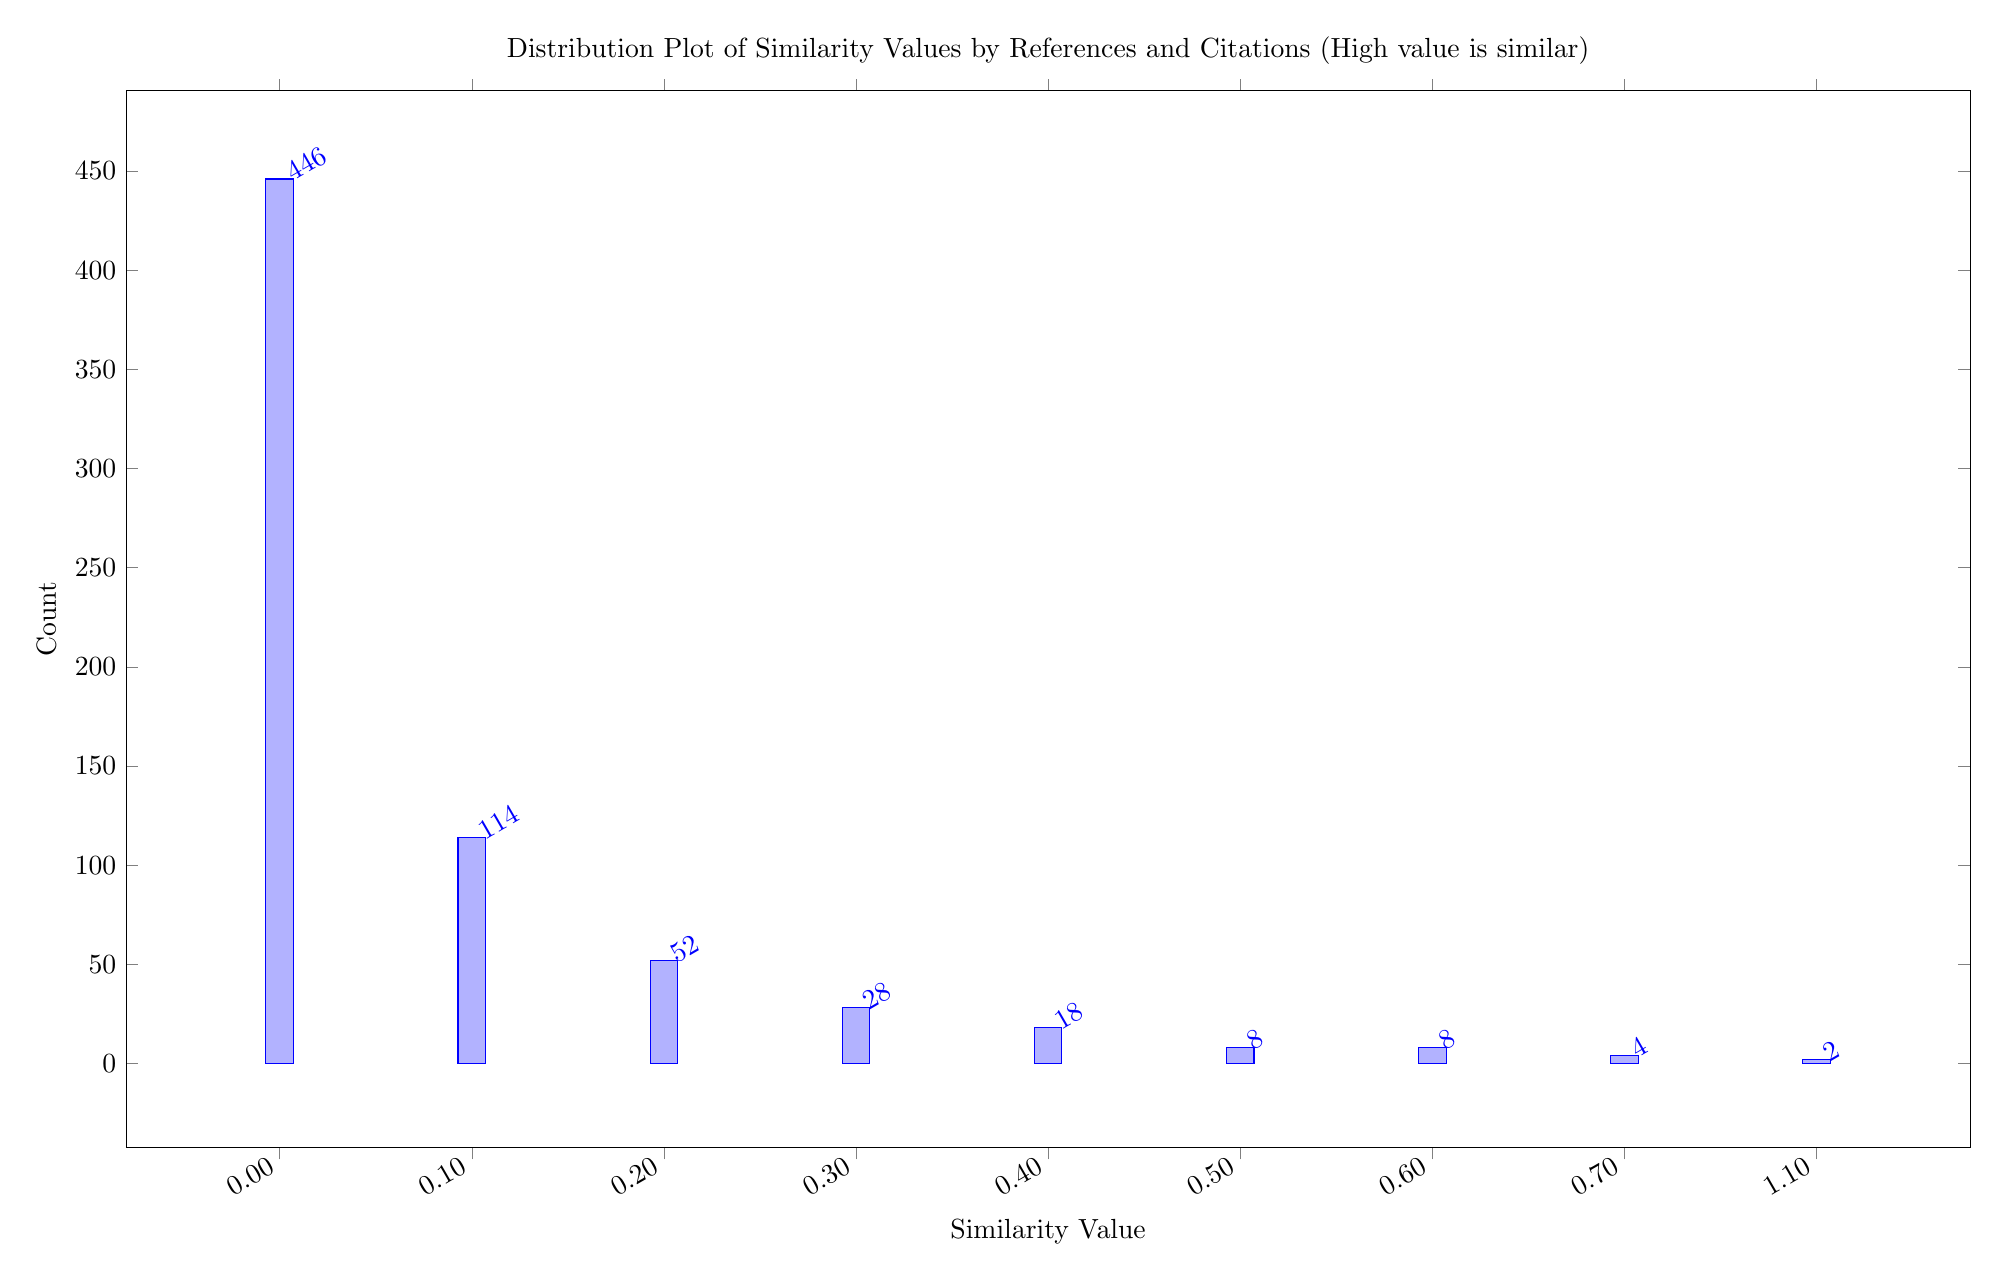
\begin{tikzpicture}
\begin{axis}[title=Distribution Plot of Similarity Values by References and Citations (High value is similar),xlabel=Similarity Value,ylabel=Count,width=25cm,height=15cm,ybar,symbolic x coords={0.00,0.10,0.20,0.30,0.40,0.50,0.60,0.70,1.10},
    xtick=data,
    nodes near coords, 
    nodes near coords align={rotate=30,anchor=west},
    x tick label style={rotate=30,anchor=east},
]
\addplot+[] coordinates {
(0.00,446.000000)
(0.10,114.000000)
(0.20,52.000000)
(0.30,28.000000)
(0.40,18.000000)
(0.50,8.000000)
(0.60,8.000000)
(0.70,4.000000)
(1.10,2.000000)
};
\end{axis}
\end{tikzpicture}

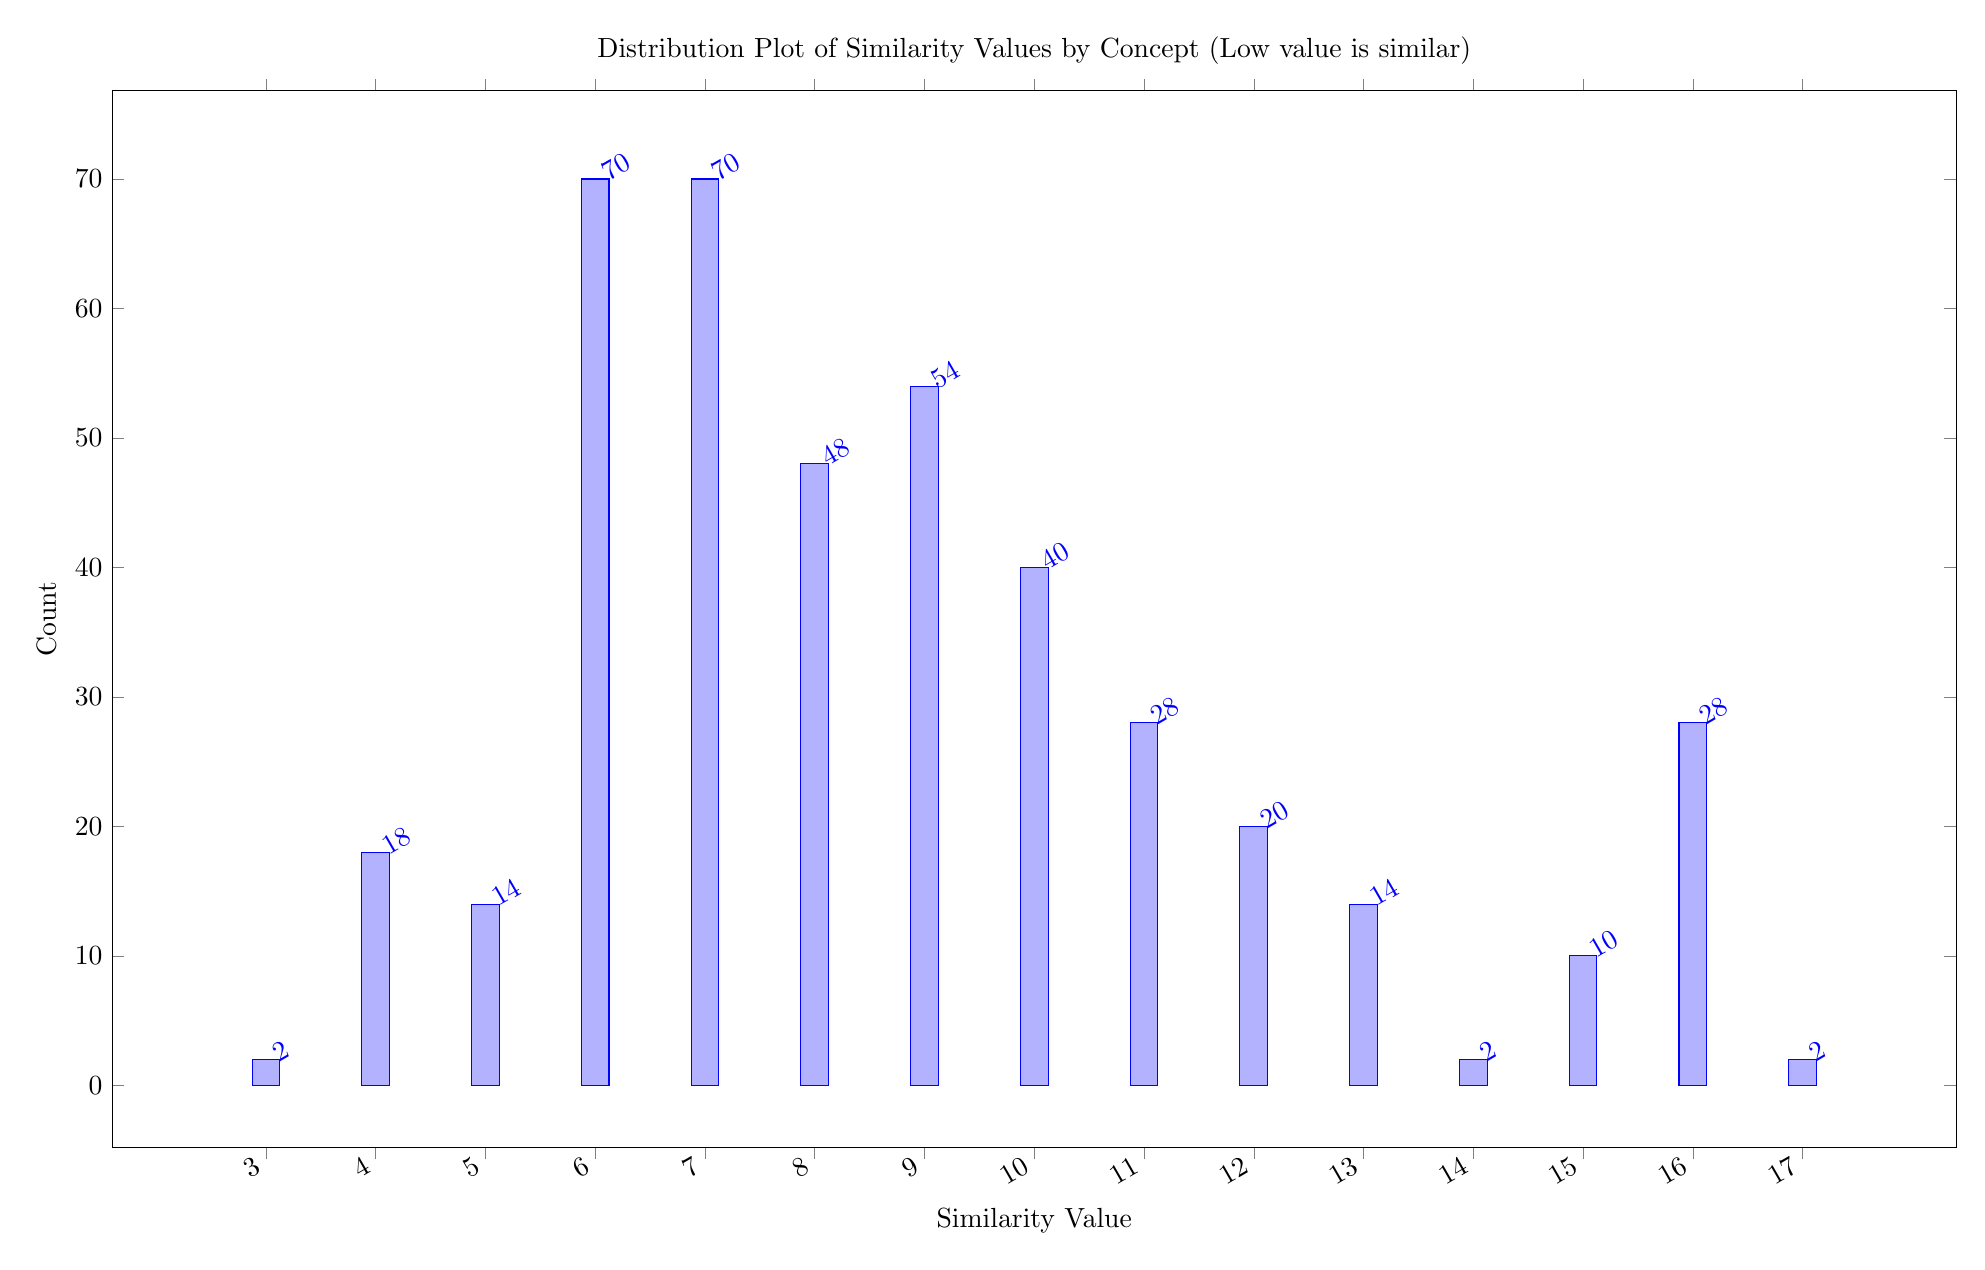
\begin{tikzpicture}
\begin{axis}[title=Distribution Plot of Similarity Values by Concept (Low value is similar),xlabel=Similarity Value,ylabel=Count,width=25cm,height=15cm,ybar,symbolic x coords={3,4,5,6,7,8,9,10,11,12,13,14,15,16,17},
    xtick=data,
    nodes near coords, 
    nodes near coords align={rotate=30,anchor=west},
    x tick label style={rotate=30,anchor=east},
]
\addplot+[] coordinates {
(3,2.000000)
(4,18.000000)
(5,14.000000)
(6,70.000000)
(7,70.000000)
(8,48.000000)
(9,54.000000)
(10,40.000000)
(11,28.000000)
(12,20.000000)
(13,14.000000)
(14,2.000000)
(15,10.000000)
(16,28.000000)
(17,2.000000)
};
\end{axis}
\end{tikzpicture}

\clearpage
\begin{figure}[htbp]
\caption{Coauthor Graph Drawn with fdp (Graphviz)}
\centering
\includegraphics[width=.6\textwidth]{../graphviz/fdp.pdf}

\end{figure}

\end{document}
